\documentclass[11pt]{article}

\usepackage[T1]{fontenc}
\usepackage[utf8]{inputenc}
\usepackage{lmodern}
\usepackage{microtype}
\usepackage{amsmath,amssymb}
\usepackage{graphicx}
\usepackage{booktabs}
\usepackage{svg}
\usepackage{caption}
\captionsetup[figure]{name=Figure,labelsep=colon}
\usepackage{fancyvrb}
\usepackage[section]{placeins}
\usepackage{float}
\usepackage{hyperref}
\usepackage{xurl}
\usepackage[nameinlink,noabbrev]{cleveref}
\usepackage[numbers]{natbib}
\usepackage[scaled=0.7]{beramono}
\usepackage{listings}

\urlstyle{tt}
\makeatletter
\g@addto@macro\UrlBreaks{\do\=\do\-\do\_\do\:\do\/\do\?\do\&\do\,\do\.\do\+}
\makeatother

\DeclareRobustCommand{\code}[1]{\begingroup\Urlmuskip=0mu plus 1mu\relax\nolinkurl{#1}\endgroup}
\renewcommand{\texttt}[1]{\code{#1}}

\title{GIAANN Proto: A General Intelligence Algorithm Artificial Neural Network for Language Modeling}
\author{\textbf{Richard Baxter}\\\small BAI Research \\\small \texttt{richard.baxter@baxterai.com}}
\date{\today}

\begin{document}
\maketitle

\begin{abstract}
General Intelligence Algorithm Artificial Neural Network (GIAANN) introduces an alternative learning algorithm to backpropagation: a dynamically growing network of features and connections for continuous learning. GIAANN Proto is an experimental implementation for language modeling.
The system constructs an excitatory database network of feature neurons organised into concept columns, incrementally updates that network during training, and performs autoregressive inference by predicting subsequent features conditioned on a seeded prompt. The neurons are sequentially activated and sensitive to the timing of their input (SANI).
This paper summarises the core ideas and provides an implementation-oriented description intended to accompany the released code.
\end{abstract}

\section{Summary}
Neural language models are commonly trained with gradient-based backpropagation and fixed-context attention mechanisms.
GIAANN explores an alternative associative memory design: an online, dynamically growing network of features and connections intended to support continuous learning and effectively unbounded context via a persistent database network.

This paper is a \emph{companion} to the codebase \texttt{github.com/bairesearch/GIAANNpy}.

\section{Background and Goals}
The project targets properties motivated by biological plausibility and continual learning, including online learning, continuous updates without catastrophic forgetting, a bias toward concept-level generalisation, and robustness to hallucination.

\section{Introduction}\label{sec:litreview}

\subsection{Semantic Networks and Relational Graphs}

Early AI systems used semantic networks (knowledge graphs) to represent relationships between concepts as nodes and links \citep{sowa_semnet}.
A semantic network is essentially a graph of interconnected nodes (concepts) and labeled edges (relations), providing a structured representation of knowledge \citep{sowa_semnet}.
Such relational graph structures enable reasoning about how entities relate to each other.
Modern approaches build on this idea with knowledge graphs and graph neural networks, which propagate information along graph edges to learn distributed representations that respect relational structure \citep{battaglia2018relational}.
This relational inductive bias allows neural models to encode entities and their relationships explicitly, improving reasoning over structured data \citep{battaglia2018relational}.

BAI’s General Intelligence Algorithm (GIA) leveraged semantic network principles.
The original GIA system constructed a relational graph of concepts from input (e.g. natural language), using methods like part-of-speech patterns and semantic relation extraction to link concepts \citep{baxterai_gia,bairesearch2017GIA}.
By pre-defining certain grammatical or semantic link types, GIA built a graph where each node (neuron or concept) connected to others based on learned relations \citep{baxterai_gia}.
An illustrative example of this relational graph structure is shown in \Cref{fig:intro-semantic-networks-relational-graph}.

\begin{figure}[htbp]
\centering
\includesvg[inkscapelatex=false,width=0.95\linewidth]{intro/BAI_GeneralAIPatentAUProv1cDRAFT_FiguresOnly_21August2012-page20}
\caption{BAI General Intelligence Algorithm (GIA) Relational concept graph illustration. Nodes coloured by type: Action reference-set delimiters (green), Condition reference-set delimiters (red), Concepts (white), Instances (cyan), Qualities (turquoise), Queries (yellow).}
\label{fig:intro-semantic-networks-relational-graph}
\end{figure}

\paragraph{Relevance to GIAANN.}

This explicit semantic network forms the backbone of knowledge in the GIA ANN.
In the GIAANN prototype, each neuron is associated with a specific concept or feature, and connections between neurons reflect probabilistic semantic or relational links (similar to edges in a knowledge graph).
This design allows the network to perform relational reasoning: when one concept neuron activates, related concept neurons can be contextually co-activated via the graph connections, mimicking how a semantic network spreads activation.

The semantic network framework provides GIAANN with a way to encode knowledge structure.
GIAANN inherits the idea of a graph-based knowledge representation, ensuring that its neural activations respect meaningful relationships rather than just statistical correlations.
In essence, GIAANN’s architecture can be seen as a neural implementation of a semantic network, where neurons are nodes and synaptic weights encode relation strengths.
This helps the model achieve more interpretable and modular knowledge representation, a key step toward general intelligence \citep{baxterai_gia,bairesearch2017GIA}.
It also means GIAANN can inherently perform relational reasoning by traversing these neural graph connections, aligning with decades of AI research on semantic networks and relational knowledge representation.

\subsection{Hopfield Networks and Emergent Sequence Prediction}
A Hopfield network is a form of recurrent neural network that serves as a content-addressable memory system \citep{hopfield1982neural}.
In a Hopfield net, all neurons are recurrently connected with symmetric weights, and the network dynamics settle to stable patterns (attractors) that represent stored memories \citep{hopfield1982neural,amit1985spinGlassNeuralNetworks}.
\citet{hopfield1982neural} showed how patterns can be stored and retrieved by the network settling to the nearest attractor state, effectively recalling a memory from partial input via energy minimisation.
A key outcome is auto-associative recall: given a cue, the network’s iterative updates cause an emergent pattern completion, retrieving the most similar stored pattern.
This emergent recall is robust to noise or incomplete data \citep{amit1985spinGlassNeuralNetworks}.
Hopfield’s work illustrated how collective dynamics of simple neuron-like units could yield memory and predictive completion of patterns without an external controller.

BAI’s Hopfield Natural Language Processing (HFNLP) is a precursor algorithm that applied a Hopfield-like associative memory to sequences (e.g. for next-word or next-neuron prediction) \citep{bairesearch2024HFNLPpy}.
In HFNLP, each ``neuron'' representing a lexical or semantic element was connected to others in a recurrent fashion.
When a concept was activated, the network would iteratively converge to the next likely concept through Hopfield dynamics.
Thus, the ``next neuron prediction'' emerged from the network’s own energy landscape: the system would settle on whichever neuron had the strongest associative link, analogous to how Hopfield nets retrieve the closest matching memory pattern.
This approach did not require a sequential control flow; instead, the sequence of activations was driven by the network’s attractor dynamics.
It is conceptually similar to Hopfield nets retrieving a sequence one item at a time, as each retrieved state provides the cue for the next.
Notably, classical Hopfield networks are static memories, but HFNLP introduced mechanisms (or iterative recall steps) to produce a temporal sequence of activations, bridging associative memory with sequence generation.

In the literature, modern developments like modern Hopfield networks (e.g. Krotov \& Hopfield 2020) and continuous Hopfield variants have increased capacity and introduced continuous states, renewing interest in Hopfield dynamics for pattern completion and even transformer-style attention mechanisms.
These works show that Hopfield associative memory can be scaled up and made differentiable, pointing toward relevance in current deep learning.
HFNLP anticipated this trend by leveraging Hopfield principles for NLP tasks.
A representative visualisation of this emergent next-neuron behaviour is shown in \Cref{fig:intro-hopfield-emergent-sequence-prediction}.

\begin{figure}[htbp]
\centering
\includesvg[inkscapelatex=false,width=0.95\linewidth]{intro/biologicalSimulationDynamicSentencesentenceIndex010Wsource013branchIndex1002sequentialSegmentIndex000}
\caption{BAI Hopfield Natural Language Processing (HFNLP) biological simulation showing emergent sequential next-neuron transitions. Network properties are coloured: Somas and dendrites (green), axons (red), synapses (yellow), activated segments/somas (cyan), activated synapses (blue), activated axons (magenta).}
\label{fig:intro-hopfield-emergent-sequence-prediction}
\end{figure}

\paragraph{Relevance to GIAANN.}
GIAANN incorporates Hopfield-like associative recall at its core.
The prototype’s neuron activations are determined in part by an energy-minimisation principle: given the current context (neuron activation levels), the next neuron to fire is the one that best satisfies the learned constraints (minimal ``energy'') of the network.
This means GIAANN can predict the next concept feature neuron in a chain without an explicit sequence model, purely by the emergent dynamics of its recurrent connections (much as a Hopfield net recalls the next part of a memory) \citep{hopfield1982neural}.
The result is that sequence generation (for reasoning or language) in GIAANN is an emergent property of the network’s learned attractor states rather than a predetermined program.
This is a distinguishing feature: whereas typical RNN/Transformer models explicitly advance time-steps, GIAANN’s sequential processing falls out from iterative relaxation to attractors.
HFNLP demonstrated a simplified version of this idea (without concept modularity), and GIAANN extends it with greater structure (as discussed below).
In summary, Hopfield’s legacy provides GIAANN a way to store and retrieve knowledge in a distributed manner and to have the next activation ``pop out'' from the network’s associative memory---a powerful form of prediction grounded in neurodynamic principles \citep{hopfield1982neural,amit1985spinGlassNeuralNetworks}.

\subsection{Sequential Activation and Multi-Compartment Neurons (SANI)}

\subsubsection{Sequential Neuron Activation}

Biological neural circuits often transmit information through spike sequences, where neurons activate one after another in precise temporal patterns.
This inspired a core property of BAI’s Sequentially Activated Neuronal Input (SANI) neural network model, the independent processesing of chains of neuron activations, as opposed to whole layers being processed sequentially \citep{bairesearch2022SANI}.
SANI networks are designed so that each neuron’s firing triggers a next neuron, creating a traversing path of activation that represents a thought or computation.
This sequential firing is more akin to how neurons in the brain might sequentially activate in a synfire chain or in language parsing (word-by-word).
An early SANI demonstration, for instance, implemented unsupervised learning of syntactic patterns, where a sequence of neuron activations corresponded to the parsed structure of a sentence (each neuron firing in turn for each word or phrase) \citep{bairesearch2022SANI, bairesearch2022SANINLPtf}.
This is in contrast to typical ANN architectures where an entire layer of neurons updates simultaneously.
The sequential activation approach enforces a temporal order and sparsity to the processing---at any given moment, only a subset of neurons is active, which then activates the next, and so on.

\subsubsection{Sequential Neuronal Input Activation}

One advantage of sequential network activation is that it mirrors the brain’s efficient use of spikes: information is carried in the timing of discrete events rather than in continuous high-dimensional vector operations.
This can be energy-efficient and interpretable (each activation is a discrete step in a reasoning chain).
However, achieving complex computation with such sparse, temporally extended activity often requires neurons to be more powerful individually---which leads to the idea of multi-compartment neuron models.
In biology, a single neuron is not a simple point neuron: it has dendritic branches that perform non-linear integrations of inputs.
These dendrites can act as semi-independent subunits, giving a single neuron the ability to detect specific spatio-temporal input patterns (almost like a tiny network within a neuron) \citep{london2005dendriticComputation}.
Recent neuromorphic research by \citet{leugering2020spiking} explicitly leveraged this, showing that multi-compartment spiking neurons (with simplified dendritic subunits) can achieve the same functionality with far fewer spikes \citep{leugering2020spiking}.
Because each neuron can do more complex processing internally, the network as a whole can fire less often: ``multi-compartment neuron models can become selective to highly specific input patterns, and thus learn to produce informative yet sparse spiking codes'' \citep{leugering2020spiking}.
In other words, a neuron with dendritic sub-components can wait until a very particular combination of signals arrives before it fires, thereby reducing unnecessary spikes while still conveying rich information per spike.

The SANI approach anticipated this benefit by effectively giving neurons more complex activation logic (sequential gating, mimicking dendritic conditions) so that only the right neuron fires at each step.

\subsubsection{Multiple Dendritic Branches}

Multi-compartment models typically also employ multiple dendritic branches, to process multiple input streams or conditions before firing \citep{leugering2020spiking, leugering2023dendritic} (see Simulated Dendritic Branches section below).

\subsubsection{Dynamically Generated Networks}

SANI also introduced dynamic generated networks \citep{bairesearch2022SANI, bairesearch2025EISANIpt} whereby neuron connectivity is dynamically generated rather established by modifying a randomly initialised network (as is common in extant artificial neural nets). This enables for a more efficient simulation of a biological substrate, restricting both memory and computation to these dynamically generated sparsely connected features.
A representative example of this incremental sequential propagation is shown in \Cref{fig:intro-sani-sequential-propagation}.

\begin{figure}[htbp]
\centering
\includesvg[inkscapelatex=false,width=0.95\linewidth]{intro/SANIgenDemoVideo1-propagationSmallL2-neuralNetIncrementalGeneration1486}
\caption{BAI Sequentially Activated Neuronal Input (SANI) incremental generation example illustrating sequential propagation through a sparse network. Network properties are coloured: neurons (blue), connections (magenta), partially activated neurons (magenta), fully activated neurons (yellow). Input layer tokens shown at top, output layer targets at bottom.}
\label{fig:intro-sani-sequential-propagation}
\end{figure}

\paragraph{Relevance to GIAANN.}
GIAANN implements SANI by incorporating multi-compartment neuron designs.
This aligns with best practices for spiking efficiency: reducing firing rate without sacrificing information is critical for energy-efficient networks \citep{leugering2020spiking}, and complex neurons provide a solution. GIAANN also incorporates dynamically generated networks, enabling for more efficient simulation of a biological substrate. Likewise, GIAANN improves on initial SANI architecture by incorporating multiple dendritic branches.

In GIAANN, each neuron’s activation may depend on converging evidence (from multiple concept connections) such that it fires only when a specific combination is met, much like a multi-compartment neuron requiring coincident inputs on its dendrites. This makes the sequential chain of activation more reliable and meaningful, as each step is a high-information event.

The sequential activation paradigm gives GIAANN a brain-like temporal dimension---processing unfolds as a series of concept neuron activations, allowing intermediate results to be interpreted step by step.
This is fundamentally different from feedforward nets and brings it closer to spiking neural networks and symbolic reasoning sequences.
By adopting multi-compartment neuron models, GIAANN’s neurons are more ``intelligent,'' each capable of complex input discrimination.
This means GIAANN can afford to have extremely sparse activity (e.g. only one neuron firing at a time) without losing computational power.
The literature on multi-compartment spiking neurons confirms that such designs can maintain performance while drastically cutting down spike events \citep{leugering2020spiking}.
GIAANN thus stands at the intersection of sequential processing (inspired by SANI and brain spike trains) and advanced neuron models (inspired by dendritic computation research), which together enable efficient, interpretable propagation of thoughts or computations one step at a time.

\subsection{Excitatory Cortical Networks and Assemblies}

Cortical neural circuits are characterised by dense recurrent excitation among nearby pyramidal neurons, forming local networks that can sustain and propagate activity.
In the absence of strong global synchronising forces, these local excitatory networks are believed to underlie the brain’s capability for pattern completion, memory replay, and sequential activation.
Experimental and theoretical studies of cortical tissue (especially in the hippocampus and neocortex) have shown that groups of excitatory neurons often form stable assemblies when learning occurs \citep{holtmaat2016assembly}.
\citet{holtmaat2016assembly} review how learning a task or memory induces specific subsets of excitatory neurons to strengthen mutual synapses, effectively ``wiring together'' into an assembly that encodes that memory or skill \citep{holtmaat2016assembly}.
Neurons are recruited into these assemblies based on their intrinsic excitability and input drive, and through synaptic plasticity they form new connections or enhance existing ones, while less useful connections are pruned \citep{yu2023synapsePruning}.
The result is an excitatory subnetwork that can ignite collectively to represent the learned information.
Such assemblies (sometimes called cell assemblies after Hebb’s theory) provide a mechanism for content-addressable storage in the brain: when a portion of the assembly is stimulated, the rest of the excitatory neurons can activate, retrieving the whole memory or initiating a learned sequence \citep{holtmaat2016assembly}.

Notably, these excitatory assemblies are constrained in space---they often correspond to local clusters of neurons (which could be within a cortical column or distributed across a few columns) that are strongly interconnected.
This ties into the concept of local connectomes or microcircuits: the specific pattern of connections among a small group of neurons can be as unique as a fingerprint for an individual (as suggested by connectomics studies), and within that local network, highly recurrent excitation plus some inhibitory shaping gives rise to preferred activation sequences.
For example, synfire chain models posit that excitatory neurons can form feedforward chains where activity propagates in order, which is a special case of an assembly arranged temporally.
More broadly, recurrent excitatory networks can exhibit attractor dynamics (settling into stable patterns) as well as sequence generation (transitioning through a series of states) depending on how weights are configured.

Evidence suggests neural inhibition rather may play a modulatory role, such as in restricting assembly activation \citep{fleming2024granule_inhibition}.
A schematic of the cortical flow in the H01 Connectome is shown in \Cref{fig:intro-excitatory-cortical-assemblies}, generated by \citet{bairesearch2025LocalConnectome} using data from \citet{shapsonCoe2021petascale,shapsonCoe2024petavoxelScience}.

\begin{figure}[htbp]
\centering
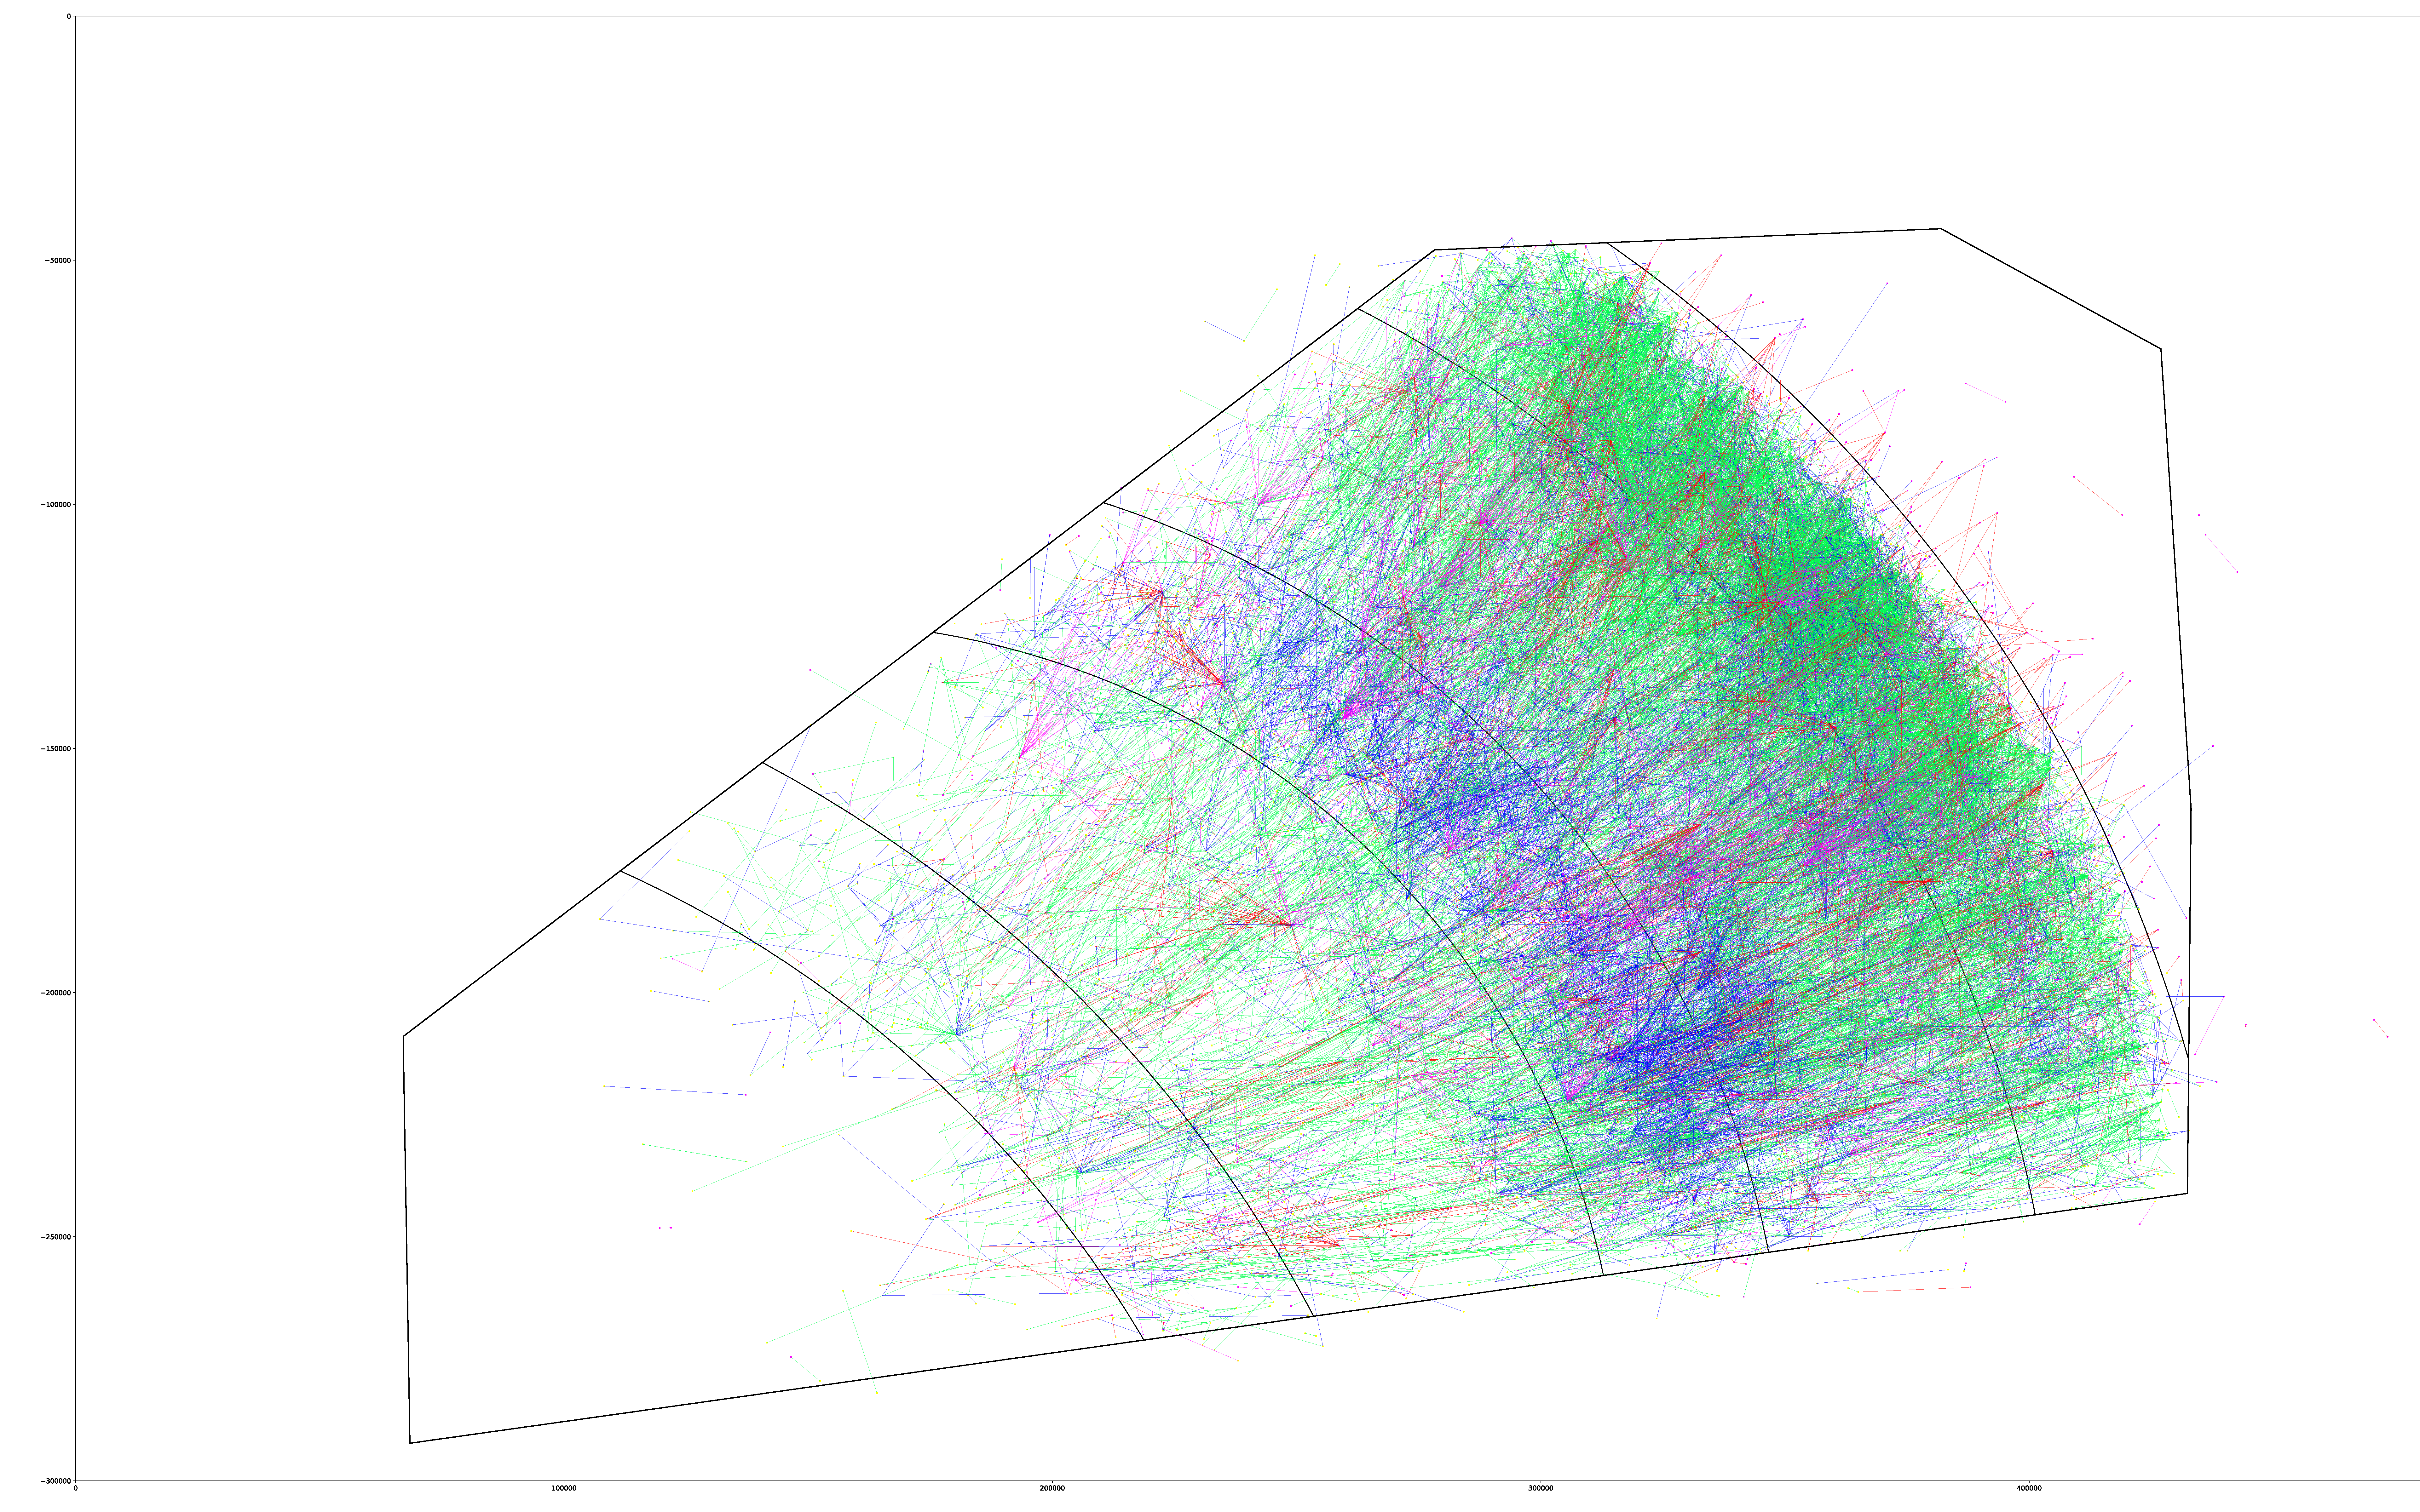
\includegraphics[width=0.95\linewidth]{intro/connections_IE_flow1_transparent_cropped.pdf}
\caption{H01 Connectome cortical network flow schematic. Network properties are coloured: excitatory neurons (yellow), inhibitory neurons (magenta), forward excitatory connections (green), backward excitatory connections (blue), forward inhibitory connections (red), backward inhibitory connections (magenta). Layers shown right to left: L1 to L7 (white matter).}
\label{fig:intro-excitatory-cortical-assemblies}
\end{figure}

\paragraph{Relevance to GIAANN.}

In GIAANN, this biological network and assembly concept is reflected in how neurons (within a concept column or across columns) are wired. See the BAI LocalConnectome repository for a detailed analysis of biological network connectivity across organisms \citep{bairesearch2025LocalConnectome}.
GIAANN emphasises excitatory-to-excitatory connections for driving the main signal flow (with inhibition playing a more modulatory role, such as resetting, normalising, and top-k selection).
This is analogous to the brain’s cortex where the heavy lifting of representation is done by excitatory pyramidal cells, and inhibitory interneurons mainly regulate timing and prevent runaway activity.
By using primarily excitatory connections, GIAANN’s dynamics rely on positive feedback loops to sustain and spread activation among related neurons---just as cortical assemblies ignite via recurrent excitation.
This design enables auto-associative recall within the network: once a partial concept is activated, the strong excitatory links can trigger the rest of the related concepts to fire in turn, completing a thought.
It also allows sequential transitions: one active neuron can excite the next intended neuron (in the learned sequence or association), enabling the chain of activation central to GIAANN’s operation.

The literature supports the efficacy of such mechanisms: recurrent excitatory circuits are thought to mediate working memory and sequence generation in cortex \citep{holtmaat2016assembly}.
Moreover, modeling studies (e.g. Hopfield nets, attractor networks, and sequence learning models) often simplify by considering only excitatory units with symmetric weights for memory storage---capturing how excitatory connectivity alone can store multiple stable states.
GIAANN leverages these principles, effectively operating as an excitatory graph of neurons wherein knowledge is stored in the connectivity.
By aligning with cortical architecture (lots of excitatory recurrence), GIAANN can achieve neural behaviors like assembly formation (group of concept neurons that commonly co-activate for a memory) and pattern completion (partial activation leads to full activation of an assembly), as described by \citet{holtmaat2016assembly}.
This biological grounding ensures that GIAANN’s learning rules and activation patterns are compatible with how real neural tissue self-organises during learning, lending plausibility and robustness to the model.

\subsection{Simulated Dendritic Branches in Neural Models}

Each biological neuron is not a point summation unit but has a complex dendritic tree that gives it computational richness.
Dendritic branches can act as non-linear subunits: they can individually perform thresholding and even spike on their own (dendritic spikes) before influencing the soma[8].
This means a single biological neuron can implement a multi-layer computation---effectively a small neural network within itself, where dendrites detect specific features and the soma integrates those results[8].
Pioneering theoretical work (e.g. by Mel and Poirazi) showed that a model neuron with passive and active dendritic compartments can perform the equivalent of an XOR or other non-linearly separable functions, and can be seen as a two-layer perceptron: inputs to separate dendrites are combined non-linearly in each branch, then the branch outputs sum at the soma (possibly triggering a spike)[8].
Such multi-compartment neuron models significantly expand the expressiveness of neural networks without adding more neurons---they add complexity within each neuron.

Recent research has explicitly incorporated dendritic computations into artificial neural networks.
For example, \citet{chavlis2025dendrites} introduced a dendritic artificial neural network where neurons had structured connectivity reflecting dendritic subunits \citep{chavlis2025dendrites}.
They demonstrated that these dendrite-enabled ANNs could achieve equal or better accuracy than traditional ones on image tasks while using far fewer parameters \citep{chavlis2025dendrites}.
The dendritic ANN was also more robust to overfitting \citep{chavlis2025dendrites}.
The authors attribute this to a different learning strategy: ``most of the nodes in dendritic ANNs respond to multiple classes, unlike classical ANNs that strive for class-specificity'' \citep{chavlis2025dendrites}.
In other words, because a neuron can compartmentalise its responses, it can participate in representing more than one category depending on which dendrite is stimulated, leading to more efficient use of neurons.
Overall, their findings suggest incorporating dendritic properties makes learning more precise, resilient, and parameter-efficient, bringing ANNs closer to the brain’s efficiency \citep{chavlis2025dendrites}.

Another line of work focuses on nonlinear integration via dendrites to discriminate input patterns.
For instance, \citet{gidon2020dendritic_ap} showed that active dendritic mechanisms in human L2/3 cortical neurons can support linearly non-separable (XOR-like) computations.
Additionally, researchers have proposed network models where each neuron has a set of learned subspace detectors (dendritic branches) that collectively determine if the neuron fires---sometimes called dendritic neural networks (e.g. the ``Dendritic CNN'' or ``DendriteNet'' models).
These models often report that for the same number of neurons, adding dendritic substructure improves task performance and noise robustness, consistent with the findings of \citet{chavlis2025dendrites}.

In addition to these rate-based and compartmentalised ANN approaches, dendrite-inspired temporal mechanisms have been studied in spiking neuron models: \citet{leugering2023dendritic} show that dendritic plateau potentials can process spike sequences across multiple time-scales \citep{leugering2023dendritic}.

In the SDBANNtf (Simulated Dendritic Branch ANN) prototype by BAI (an early TensorFlow implementation focusing on dendrites) \citep{bairesearch2023SDBANNtf}, the idea was to give each artificial neuron multiple internal ``branch'' computations.
Each branch would receive a subset of inputs and produce a sub-output; the neuron fires only if one or more branches reach a threshold. Related NLP experiments are provided in the SDBNLPpt (Simulated Dendritic Branch NLP) prototype \citep{bairesearch2023SDBNLPpt}.
This mimics how real neurons might require a strong input to one dendrite (or coincident inputs to that branch) to fire, rather than summing weak inputs from everywhere.
It creates a more disjunctive or condition-specific firing behavior, as opposed to the purely additive behavior of standard neurons.

\paragraph{Relevance to GIAANN.}
GIAANN incorporates simulated dendritic branch logic into its neurons, following these research insights.
Concretely, each concept neuron in GIAANN can have multiple input streams or conditions that must be met---analogous to multiple dendritic branches that each detect a particular conjunction of features.
This allows GIAANN neurons to be highly selective: they might only activate for a concept if certain context features come into branch A or B, for example. (Although branch interaction is not currently enabled, they could also only activate if certain context features from different branches A and B coincide).
This selectivity is exactly what multi-compartment neurons enable: ``selective to highly specific input patterns, producing sparse spiking codes''[9].
Thus GIAANN’s neurons do not fire for every slight stimulus; they await a meaningful pattern, reducing spurious activations.
As a result, the network’s overall activity is sparse and information-rich, improving efficiency and interpretability.

By using dendritic subunits, GIAANN neurons can participate in multiple representations.
For instance, the same neuron might contribute to two different concepts depending on which dendrite is activated (similar to how one neuron in dendritic-ANN responded to multiple classes) \citep{chavlis2025dendrites}.
This aligns with the brain’s reuse of neurons across contexts and helps GIAANN avoid combinatorial explosion of neurons for every concept.
It also reinforces the idea of concept columns: within a column (see next section), neurons might share input branches for column-specific features, while other branches capture cross-column context, thereby integrating local and global information.
The literature strongly backs the inclusion of dendritic mechanisms as a path to more powerful and brain-like ANNs, and GIAANN stands on that frontier by explicitly baking in dendritic branch computations into its architecture.

\subsection{Semantic Encoding in Single Neurons}

One of the striking findings in neuroscience is that single neurons can encode high-level, abstract information---sometimes very specifically.
Classic examples are the so-called ``concept cells'' discovered in the human medial temporal lobe (MTL).
\citet{quiroga2005concept} famously reported neurons that respond selectively to different images of the same person (e.g. Jennifer Aniston) and even to the written or spoken name of that person.
These neurons fire for a particular concept regardless of how it’s presented---a property known as invariant representation.
The selectivity is extremely sparse (out of tens of millions of neurons, only a handful might fire for that concept) and explicit (the neuron’s firing strongly indicates the presence of that concept) \citep{quianQuiroga2012conceptCells}.
This led to discussion of ``grandmother cells''---not literally one neuron per concept, but a spectrum where some neurons lie at the explicit end of representation.
Further research by \citet{quianQuiroga2012conceptCells} reinforced that concept cells are part of a distributed but sparse assembly coding for an item, and they likely play a role in memory (linking concepts together, since the hippocampal formation is involved in memory).
These findings demonstrated that semantic encoding can be achieved at the single-cell level in a highly selective manner \citep{quiroga2005concept}.

More recently, \citet{jamali2024semantic_encoding} provided unprecedented insight into semantic encoding in the human cortex \citep{jamali2024semantic_encoding}.
They recorded from single neurons in the language-dominant prefrontal cortex of patients listening to natural speech.
They found that individual neurons showed selectivity for specific word meanings---for example, a neuron might fire for any word related to a particular semantic category or concept \citep{jamali2024semantic_encoding}.
These neurons could even distinguish real words from pseudowords, indicating a true semantic discrimination, not just sound or frequency \citep{jamali2024semantic_encoding}.
Importantly, the firing of these neurons was context-dependent: the same word could elicit different neural responses depending on the sentence context, meaning that neurons were encoding semantic information in a flexible way, sensitive to how meaning changes with context \citep{jamali2024semantic_encoding}.
They also found that ensembles of such neurons encoded the hierarchical structure of meaning representations in their firing patterns \citep{jamali2024semantic_encoding}.
In summary, this study revealed ``a fine-scale cortical representation of semantic information by individual neurons,'' with neurons dynamically reflecting the meaning of words in context \citep{jamali2024semantic_encoding}.
This is direct evidence of single-neuron semantics in the cortex, complementing the concept cells of MTL with more language-oriented examples in the prefrontal cortex.

These results, combined with earlier findings, suggest a continuum between fully distributed representations (many neurons share in representing a concept) and extremely sparse ones (a neuron or a small set encodes a concept).
Not all neurons are concept cells, but the existence of such cells implies that a neural system can assign distinct semantics to individual units.
This is an appealing property for interpretable AI models---if each artificial neuron corresponded to a human-comprehensible concept, the network’s reasoning would be more transparent.
Traditional deep networks, however, tend to use distributed representations; no single unit cleanly corresponds to a high-level concept (with some exceptions in deep vision models where certain units detect specific objects or features).
There has been growing interest in disentangled representations in AI---where dimensions or units correspond to meaningful factors of variation.
The brain’s concept cells are like an existence proof that disentangled (or at least highly sparse localised) representation is possible and useful.

\paragraph{Relevance to GIAANN.}
GIAANN explicitly embraces the idea of neurons as semantic encoders.
It is built so that each neuron (or a small coherent group of neurons) represents a distinct concept, feature, or memory element.
This design is in line with the findings of concept cells and Jamali et al.’s semantic cells.
By allocating neurons to specific meanings, GIAANN ensures that activation of that neuron signals the presence of that meaning in the current context---much like a concept cell firing signifies a particular person or thing is being thought about \citep{quianQuiroga2012conceptCells,quiroga2005concept}.
GIAANN’s training and architecture encourage this localisation: learning rules are constrained so that neurons develop sharp selectivity (via sparse Hebbian updates) rather than distributed entangled representations.
The concept columns in GIAANN (discussed next) also foster this, by grouping neurons by topic/domain which reduces overlap of unrelated features in the same neurons.

By mirroring single-neuron semantic coding, GIAANN gains interpretability (one can inspect which concept neurons fired to understand its ``thought process'') and potentially leverages the brain’s efficient encoding (sparse firing, as only the relevant concept neurons fire, saving energy/computation).
It also allows contextual modulation of semantics: because GIAANN’s neurons can interact (via lateral modulation), the activation of a concept neuron can reflect context, similar to Jamali et al.’s observation that neuron responses to words depend on sentence context \citep{jamali2024semantic_encoding}.
For example, a ``bank'' neuron might only fire if disambiguating context indicates finance (and stay quiet if the context is ``river bank'', allowing a different set of neurons to fire).
This kind of context-sensitive concept representation is exactly what the human neurons exhibited and is a targeted feature for GIAANN.

In summary, neuroscience has shown that single neurons can carry high-level meaning, and GIAANN capitalises on this by structuring its representational scheme around neurons-as-concepts, a departure from most contemporary ANN models. Although its present implementation exhibits limited semantic overloading during training (noun homonymy, e.g. ``bank''), this does not cause significant confliction during inference due to the dominance of contextual neuronal representations.

\subsection{Cortical Columns and Modular Organisation}
The neocortex is often described as a repetitive lattice of cortical columns---vertically arranged microcircuits ($\sim$50--100\,\textmu{}m wide minicolumns and larger $\sim$0.5--1\,mm macrocolumns) that each perform a sort of canonical computation.
\citet{mountcastle1997columnar} originally proposed the columnar organisation as a fundamental principle: neurons in a small column respond to similar features or input from the same receptive field.
More recent theories, like Jeff Hawkins’ Thousand Brains Theory, dramatically expand the role of columns, suggesting that each cortical column learns a complete model of objects or concepts from its perspective \citep{hawkins2011htm}.
Rather than information being siloed to a single part of the hierarchy, each column creates an internal representation of whole objects and then columns vote or consensus-build to form our singular perception \citep{hawkins2011htm}.
In this view, intelligence emerges from an army of parallel experts (columns), each of which is modeling the world in slightly different ways (e.g., each column might be anchored to a different sensor or reference frame).
Long-range horizontal connections allow these columns to synchronise on an agreed interpretation \citep{hawkins2011htm}.
Hawkins’ Hierarchical Temporal Memory (HTM) algorithm was an attempt to implement key aspects of cortical columns in a computational model.
HTM uses sparse distributed representations and organises neurons into minicolumns and layers that mimic cortical layering \citep{hawkins2011htm}.
Notably, in HTM each minicolumn’s cells learn temporal sequences and make predictions: if an input sequence is recognised, one cell in a minicolumn will enter a predictive state (like a guess for the next input) \citep{hawkins2011htm}.
Only one cell per minicolumn fires for any given context, enforcing a sparse code.
This is analogous to the idea that in a cortical column, only a small fraction of cells are active at once, representing a particular feature in a particular context.

HTM and related models demonstrate how modular organisation (columns, layers) plus sparse coding and local learning rules (Hebbian, no backprop) can learn sequences and make predictions in a streaming manner \citep{hawkins2011htm,numenta2019_htm_guide}.
While HTM did not become mainstream in machine learning, it captured brain-like attributes: continuous learning, temporal context, and modular structure.
It is essentially a column-oriented view of computation, differing from traditional deep networks that use homogeneous layers.
Another relevant concept from neuroscience is that columns may correspond to functional units or maps (e.g., orientation columns in visual cortex, where each column handles a particular orientation of visual edge).
Holtmaat \& Caroni’s assembly formation could be seen in the column context: if learning recruits an assembly of neurons, often those neurons are spatially proximate (due to local recurrent connectivity), possibly within a cortical column or a couple of neighboring columns[10].
Thus, an assembly might actually be a ``column-sized'' group encoding a memory.
This links columns to the idea of local learning and memory encoding, reinforcing that columns are not just anatomical structures but computational modules that can hold discrete pieces of information.

In modern deep learning, an interesting parallel to cortical columns is the use of dedicated substrate experts such as multiple attention heads in Transformer architectures.
A Transformer doesn’t have physical columns, but each attention head can be thought of as focusing on a different subspace or aspect of the input.
\citet{vaswani2017attention} introduced multi-head self-attention specifically to allow the model to capture different relationships in the data simultaneously \citep{vaswani2017attention}.
``Each attention head learns different projections of Q, K, V, allowing the model to capture different aspects of the relationships between words in the sequence simultaneously'' \citep{vaswani2017attention}.
In essence, each head is somewhat analogous to a mini-module that extracts a particular kind of pattern (for example, head~1 might attend to syntactic structure, head~2 to coreference, head~3 to anaphora resolution, etc., in an NLP context).
After processing, the outputs of all heads are combined.
This bears similarity to the idea of multiple cortical columns each processing the input (or parts of it) in parallel and then integrating their findings.
The analogy is not perfect---Transformer heads share most of their surrounding network---but conceptually, dividing representational resources into parallel ``columns'' that specialise is a common strategy in both the brain and advanced ANN designs.

\citet{bahdanau2015neural} likewise introduced the idea of dividing a context into distinct subspaces of tokens, whereby the processing of each token can proceed somewhat invariant to the absolute position of the token in its context. While these subspaces may primarily form syntactical priors at lower layers (via attention), and semantic priors at intermediate layers (via attention), they form specific concepts at higher layers and interact with other specific concepts (via attention). As such, this segregated information retentic/combinatory property of the transformer architecture also resembles columnar processing of tokens within sequences.

\paragraph{Relevance to GIAANN.}
GIAANN explicitly implements a form of concept-wise modularity that can be seen as artificial cortical columns.
Neurons in GIAANN are organised into concept columns, each column devoted to a group of related features or a domain of knowledge (noun).
For example, one column might represent dogs, another cats, another trees (analogous to how the brain might have columns or patches for different categories of information).
Within a concept column, neurons share certain inputs or dendritic branches (the ``common context'' of that column), and they compete or cooperate to represent specific instances of that concept.
This is much like HTM’s minicolumns where only one cell is active per context---in GIAANN, only one neuron per concept column fires at a time (a winner-take-all style competition; see \citealt{maass2000winnerTakeAll}), representing the specific concept active in the current thought.
By segregating neurons into columns, GIAANN ensures that unrelated concepts do not directly compete; competition is localised, which simplifies learning (reduces interference) and improves interpretability (one can decode a network state by picking at most one active neuron from each column, yielding a set of active concepts).
The columnar design also allows GIAANN to scale: new knowledge can be added by adding neurons to existing columns or new columns, without disrupting learned representations in other columns (mitigating catastrophic forgetting via modularity).

GIAANN’s concept columns resonate with Hawkins’ theory---each column holds a model of a piece of the world (like one facet of an object or one type of entity), and collectively these models contribute to a coherent perception or solution.
The network’s long-range (inter-column) connections let columns influence each other (ensuring consistency, much as cortical long-range fibers enable columns to vote and agree) \citep{hawkins2011htm}.
This means GIAANN can achieve an ensemble effect: multiple ``experts'' (columns) each supply part of the interpretation of input, and their interaction yields a rich understanding.
In the context of multi-head attention, GIAANN’s columns can be viewed analogously---each column might attend to a different aspect of the input or context, and by having multiple such columns active (in sequence or in parallel), GIAANN covers a broad combinatorial space of possibilities without conflating them in one monolithic representation \citep{vaswani2017attention}.

Finally, because each column in GIAANN is like a micro-network with its own localised learning, the system aligns with the brain’s developmental and functional segregation---it’s easier to train (each column can self-organise with minimal interference) and it’s robust (damage to one column only affects that aspect of processing, not everything).
This is a marked difference from prior BAI models like HFNLP \citep{bairesearch2024HFNLPpy}, which lacked this columnar separation and thus had all neurons in one big pool competing.
GIAANN, by introducing concept columns, moves from a single Hopfield-memory to multiple overlapping Hopfield-like modules, which is a novel synthesis of columnar neuroscience ideas and modern neural network design.


\section{Discussion}

\subsection{Synthesis and Novelty}

In the introduction we presented prior work and how it informed GIAANN, focusing on background and synthesis.
Here, in the discussion we critically analyse how GIAANN diverges from those priors and what unique contributions it makes.

The GIAANN prototype brings together all the above themes into a unified architecture, and in doing so, it differs from prior works in significant ways while also addressing some of their limitations.
A key distinguishing feature is GIAANN’s explicit combination of multiple brain-inspired mechanisms in one system.
Where most previous models or theories focused on one or two of these aspects in isolation (e.g., HTM on columns and sequences, or dendritic ANNs on neuron substructures, or Hopfield nets on associative memory), GIAANN integrates semantic graphs, Hopfield dynamics, sequential spiking, dendritic compartments, concept cells, and columnar organisation into a single algorithmic framework.
This integrative approach is itself novel---it treats these concepts not as disparate research threads but as synergistic components of general intelligence.

Concretely, compared to its direct precursor, HFNLP \citep{bairesearch2024HFNLPpy}, GIAANN introduces Concept Columns.
HFNLP demonstrated that a Hopfield-like network could autonomously predict the next element in a sequence (particularly in language processing) via associative recall, but it treated the neuron population as largely homogeneous.
There was no structural separation for different types of information---all ``concepts'' lived in one recurrent pool, meaning the network struggled with interference and scaling (adding more concepts would eventually confuse the associative memory).
GIAANN overcomes this by dividing the neural substrate into columns, each handling a subset of the knowledge domain.
This means that when predicting the next neuron, GIAANN does not search the entire space blindly; it knows, for instance, that if the last active neuron was in a ``subject'' column, the next likely neuron might be in a related ``object'' column.
This structured traversal is far more scalable and mirrors how language or reasoning often has slots or roles (subject, predicate, object; or context, entity, attribute) that constrain what comes next.
In essence, GIAANN adds a contextual guide to the Hopfield recall: the semantic network (relational graph) plus column structure narrows the attractor search to sensible regions, thus solving one shortcoming of pure Hopfield nets, which can get spurious memories or require full connectivity.
The result is more reliable and interpretable sequence generation.

Relative to HTM and other cortical column models, GIAANN is less biologically literal in some ways (HTM models detailed minicolumns, layers, etc.), but it goes beyond them by incorporating full semantics and learning of explicit concepts.
HTM, for example, did not assign semantic labels to columns; it learned generic spatial-temporal patterns.
GIAANN builds in a semantic network from the start, ensuring each column/neuron has a meaning in human-understandable terms (at least after training).
This marriage of symbolic semantic structures (graphs) with sub-symbolic neural dynamics is reminiscent of neurosymbolic AI, but GIAANN does it in a tightly integrated, brain-inspired manner rather than attaching a logic engine onto a neural net.
The result is a system that can store knowledge (relations, facts) and process (chain through them) coherently.
Moreover, GIAANN’s use of dendritic logic within neurons is something HTM’s neuron model (though more complex than a perceptron) did not explore in depth.
Thus, GIAANN’s neurons are more powerful, potentially reducing the number of neurons needed and enabling the network to handle more complexity with sparse activity.

Against the backdrop of modern deep learning (e.g. Transformers), GIAANN stands out by eschewing backpropagation and dense continuous representations.
Instead, it relies on local learning rules (Hebbian) and highly sparse, event-driven computation.
This means GIAANN might not reach the performance of a Transformer on benchmark datasets and evaluation metrics, however, it offers advantages in interpretability, incremental learning, and energy efficiency (and experiments are indicative of consistent scaling).
Every activation in GIAANN can be traced to a concept, every connection to a relation---a transparency that is largely missing in black-box deep nets.
And whereas Transformers require enormous training data and then struggle with one-shot or continual learning, GIAANN (like the brain) can potentially incorporate new knowledge by adjusting a few connections in the semantic graph or adding a new neuron/column, without retraining the whole network.
This addresses the plasticity-stability dilemma in a structural way: knowledge is compartmentalised, so new learning in one column minimally interferes with established memories in others.

\subsection{Limitations}

It is important to note that while GIAANN draws on biology, it is not a direct simulation of the brain but rather a brain-inspired algorithm.
Consequently, some differences exist: for instance, real cortical columns may not each hold a distinct ontology of a concept---the brain’s columns may be more sensorily grounded whereas GIAANN’s may be more abstract and conceptual.
Also, inhibitory interneurons are critical in cortex for shaping activity; GIAANN currently emphasises excitatory drives with simplified global inhibition or as a mechanism for restricting prediction targets (exclusive top-1 selection, akin to winner-take-all \citep{maass2000winnerTakeAll}).
Additionally, GIAANN’s reliance on a predefined semantic cues (POS identification for concept column delimitation) could be seen as a limitation compared to deep learning models that learn representations purely from data.
However, one might argue GIAANN is simply incorporating prior knowledge (thing/relation distinction) which is a strength, not a weakness, especially for AGI aspirations.

\subsection{Conclusion}

In summary, GIAANN represents a novel synthesis that addresses shortcomings in prior art: it tackles the scaling issue of Hopfield memories by structuring them into columns; it improves interpretability and incremental learning relative to end-to-end deep nets; it increases neuron computational capacity instead of sheer quantity, aligning with energy constraints; and it grounds neural processing in explicit semantics, narrowing the gap between sub-symbolic neural nets and symbolic reasoning.
Its design is unorthodox in the contemporary ML landscape, but it hews closely to many cognitive and neuro principles, potentially offering a path to more general, human-like intelligence in machines.
As such, GIAANN differs from prior models: it is neither purely a Hopfield net, nor an HTM, nor a standard ANN, but an amalgam that leverages their strengths while mitigating their weaknesses.
The result is an architecture well-suited to embody understanding, reasoning, and learning in a way that is both computationally efficient and interpretable---a promising development in the quest for general AI.

\section{Development}\label{sec:development}

GIAANN was developed as a neuralisation of GIA: the symbolic graph machinery of GIA was retained
(substance/action/condition structure, reference delimiters, and concept-level composition), but
execution was shifted from explicit symbolic traversal to sparse neural activation and local synaptic
updates \citep{baxterai_gia,bairesearch2017GIA}. The objective was to preserve GIA's interpretable
semantics while introducing brain-inspired mechanisms for continual learning, scalable memory, and
emergent sequence prediction.

\subsection{GIA History}

The General Intelligence Algorithm (GIA) originated as an explicitly symbolic architecture and was
released publicly through the original OpenGIA SourceForge codebase in 2012
\citep{bairesearch2022OpenGIAsourceforge} (and GitHub in 2017 \citep{bairesearch2017GIA}). That implementation established the core representational
scheme later retained by GIAANN: compositional semantic structures built from substance, action, and
condition roles; explicit reference delimiters for binding and lookup; and graph-based mechanisms for
storing and traversing concept/event relations.

The preliminary Australian provisional patent drafts (1B and 1C) documented this early design as a
general method and computer-system formulation, clarifying the intended scope and operational
workflow of the algorithm \citep{bairesearch2022giaPatentAUprovisional1B,bairesearch2022giaPatentAUprovisional1C}.
Together, the released code and patent drafts provide the historical baseline for GIA as a
semantic-first, interpretable reasoning system, from which the later neuralisation into GIAANN was
developed.

\subsection{From GIA to a Brain-Inspired Neural Substrate}

The early architecture separated a semantic concept network from an episodic instance network,
reflecting GIA's distinction between stable concept knowledge and context-bound events. Over
subsequent revisions, this evolved from a rigid instance ledger toward synaptic event encoding:
episodes became increasingly represented by connection strengths and activation traces over concept
neurons. This was a key transition from symbolic storage to neural memory while keeping the same
conceptual ontology.

Known brain functioning informed each major design choice. Sensory-like feature streams (auditory
and visual) were treated as lower-level inputs converging into a concept integration pathway.
Reference generation (binary/temporal coding) played a thalamus-like indexing role for binding
distributed features into addressable concepts. Later, cortical columnar ideas motivated semantic
concept columns, and sparse competition with selective firing aligned with winner-take-all and
dendritic-style conditional integration \citep{mountcastle1997columnar,london2005dendriticComputation,maass2000winnerTakeAll}.

\subsection{Chronological Architecture Milestones}

The Appendix \Cref{subsec:appendix-giaann-development} GIAANN Development diagrams show the progression below (oldest to newest):

\begin{itemize}
    \item \Cref{fig:dev-2017-initial-core}: initial symbolic core with semantic concepts, episodic instances, and binary reference coding over axonal conduits.
    \item \Cref{fig:dev-2019-event-retrieval}: event retrieval refinement with feedback encoding and rate-coded lookup from partial cues (subject/action/object/place-time subsets).
    \item \Cref{fig:dev-2021-biomodel-mapping}: explicit bio-model mapping across thalamus, cortex, striatum, and limbic/hippocampal roles, including design rationale and predicted serial-access constraints.
    \item \Cref{fig:dev-2021-synaptic-encoding}: transition toward storing episodic information in synapses associated with substance/concept neurons, with a consolidated concept-integrator/reference-generator pathway.
    \item \Cref{fig:dev-2024-columns-routing}: introduction of semantic concept columns and temporary unassociated nodes, with inter-column delimiter features (verbs and prepositions) used as routing constraints.
    \item \Cref{fig:dev-2024-feature-split-gating}: explicit split between inter-column and intra-column features (e.g., qualities), plus syntactic-validity gating so invalid nodes/links remain weak or temporary.
\end{itemize}

\subsection{Resulting GIAANN Design}

Across these stages, GIAANN preserved GIA's semantic compositionality while increasingly grounding
computation in biologically inspired principles: modular columns, sparse competitive activation,
temporally indexed references, and distributed synaptic memory. The result is not a purely symbolic
parser and not a standard backpropagation ANN, but a semantic-first, brain-inspired architecture for
interpretable continual learning and sequence-level reasoning.

\subsection{GIAANN Proto Development}

A full prompt-level natural language specification of GIAANN Proto is provided in Appendix \Cref{subsec:appendix-giaann-proto-spec} (\texttt{dev/GIAANNproto1.nlc}). All debugging prompts are omitted (OP is provided). Manually programmed items have prefix \texttt{MANUAL}.

The major public version of the prototype is \texttt{1}, and the minor public versions are alphabetised (e.g. \texttt{1k}). The large language model used to assist programming the natural language code is provided for each minor public version. There was a significant period of time between the release of OpenAI o1 preview \citep{openai2024o1preview} and GPT-5-Codex \citep{openai2025gpt5codex, openai2025gpt51codex} where all programming had to be performed manually due to the complexity of both the algorithm and the codebase. The majority of programming could be performed in natural language with assistance from GPT-5.2-Codex+ \citep{openai2025gpt52codex, openai2026gpt53codex, openai2026gpt54codex}.

\section{Algorithm}

The GIA ANN prototype is a concept--feature neural database that learns from text sequences and predicts next tokens by activating connected features. It treats nouns as concept columns, and every other token as a feature neuron within those columns. The algorithm is designed for online, unbatched learning, and stores most of its state in sparse tensors for scalability.

\begin{center}
\includesvg[width=\linewidth]{demo/GIAANNproto1cAllColumnsTrainSequenceIndex005}
\par\smallskip
\refstepcounter{figure}\label{fig:giaannproto1c_allcolumns_train_005}
\textbf{Figure~\thefigure:} Example all-columns network visualisation during training.
\end{center}

\subsection{Core Data Structures}
\begin{itemize}
	\item \textbf{Concept columns:} a dynamic dictionary mapping concept lemmas to column indices ($c$). Each column has a prime concept neuron at a fixed feature index.
	\item \textbf{Feature dictionary:} a dynamic dictionary mapping feature words to feature indices ($f$). Features are words (not lemmas) and are shared across columns.
	\item \textbf{Observed columns:} per-sequence objects that hold the sparse feature neuron tensors and feature connection tensors for each concept column seen in the sequence.
	\item \textbf{SequenceObservedColumns:} a per-sequence view that stacks the observed columns into dense or sparse tensors of shape (properties$\times$branches$\times$segments$\times$columns$\times$features), plus a matching feature--connection tensor.
	\item \textbf{Properties:} strength, permanence, activation, time, POS, and optional minimum word distance. Which properties exist is controlled by configuration.
	\item \textbf{SANI segments:} each dendritic branch is segmented to encode sequential ordering. Segment indices are assigned by column distance, feature distance, or both.
\end{itemize}

\subsection{Preprocessing and Column Segmentation}
\begin{enumerate}
	\item \textbf{Sequence construction:} text is parsed with spaCy; sequences are either single sentences or multi-sentence bundles. Empty or too-short sequences are skipped.
	\item \textbf{Token normalisation:} tokens are lowercased, lemmatised, and optionally preprocessed to combine consecutive nouns or hyphenated noun phrases.
	\item \textbf{Concept detection:} nouns are detected via POS rules (or the full POS dictionary); these lemmas define concept columns.
	\item \textbf{Delimiter detection:} reference set delimiters are detected by POS, tag, or word lists. Deterministic delimiters take priority over probabilistic ones.
	\item \textbf{Column assignment:} tokens are assigned to concept columns by choosing the rightmost delimiter between adjacent concept tokens. If no delimiter exists, the sequence is skipped (training) or inference is aborted (prediction).
\end{enumerate}

\subsection{Training Algorithm}
\begin{enumerate}
	\item \textbf{First pass (concept growth):} scan the sequence and add new concept lemmas to the concept column dictionary. If $c$ grows, resize global feature tensors.
	\item \textbf{Feature discovery:} scan the sequence for non-concept tokens and add new feature words to the feature dictionary. If $f$ grows, expand all feature tensors.
	\item \textbf{Observed column loading:} for each concept in the sequence, load or create its observed column object and refresh its arrays to the current $c$ and $f$.
	\item \textbf{Column segmentation:} compute per-concept token spans and build a token-to-column assignment list.
	\item \textbf{Feature activation tensor:} for each concept instance, mark active feature neurons inside the column span. Assign dendritic branches (optionally randomized) and SANI segments based on column or feature distance.
	\item \textbf{Connection activation tensor:} create directed connections between active features, enforcing forward word order and column order. Optionally enforce direct connections (adjacent tokens only).
	\item \textbf{Update rule:}
	\begin{itemize}
		\item Strength is incremented for active features and connections (with optional normalisation and POS-dependent scaling).
		\item Permanence is incremented for active features/connections and can be decremented for inactive ones.
		\item Activation traces and time properties are reset or updated as configured.
		\item POS and minimum word distance properties are recorded for active items.
	\end{itemize}
	\item \textbf{Commit:} merge sequence tensors back into observed columns, save updated columns and dictionaries to disk, and optionally draw the network.
\end{enumerate}

\subsection{Inference Algorithm (Seed + Prediction)}
\begin{enumerate}
	\item \textbf{Seed phase:} use the same prediction pipeline as normal inference, but force the selected feature to be the target token. This seeds the activation state.
	\item \textbf{Activation state:} use global sparse activation tensors (and optional connection tensors) as the working state for predictions.
	\item \textbf{Sequential gating (SANI):} apply sequential activation rules so a segment can only fire if the previous segment is active.
	\item \textbf{Delimiter constraints:} if the current active node is a reference-set delimiter, constrain the next prediction to delimiter-compatible nodes or external columns.
	\item \textbf{Time-based biasing:} optionally adjust segment activations based on last activation time relative to the expected segment index.
	\item \textbf{Candidate selection:}
	\begin{itemize}
		\item If beam search is enabled, expand beams to a fixed depth and width, scoring by activation and connection strength.
		\item Otherwise, select the single best node from the current activation map.
	\end{itemize}
	\item \textbf{State update:} activate the chosen node, update activation traces and time properties, and propagate its outgoing connections to update the next step.
	\item \textbf{Evaluation:} optionally compare predictions to the target token and log mismatches.
\end{enumerate}

\subsection{Beam Search (Optional)}
\begin{itemize}
	\item Each beam holds a cloned activation state (feature activations, optional connection activations, and time properties).
	\item Candidate nodes are filtered by constraint mode, connected-column constraints, and activation thresholds.
	\item Beam scoring can use activation gain, connection strength, or both. The final prediction is the first action of the highest-scoring beam.
\end{itemize}

\subsection{Persistence and Visualisation}
\begin{itemize}
	\item Each observed column is stored on disk with its sparse tensors and feature mappings.
	\item Global feature neuron tensors and concept/feature dictionaries are saved at configurable intervals.
	\item The visualiser renders concept columns, feature nodes, and connections with colour schemes for segments, branches, POS types, or delimiters.
\end{itemize}


\section{Implementation}

\subsection{GIAANNproto\_globalDefs.py}
\begin{itemize}
	\item Central configuration for all training, inference, memory, and visualisation options (e.g., \texttt{useInference}, \texttt{useSANI}, \texttt{conceptColumnsDelimitByPOS}).
	\item Defines tensor property layout (strength, permanence, activation, time, POS, min-distance) and derives array indices and segment counts from seed length and SANI settings.
	\item Sets dataset, device, and performance toggles, plus debug and draw flags used across the codebase.
\end{itemize}

\subsection{GIAANNproto\_main.py}
\begin{itemize}
	\item Entry point that loads the dataset, initialises spaCy, and orchestrates training vs. inference loops.
	\item Implements the per-article and per-sequence pipeline: preprocessing, concept detection, observed column loading, sequence tensor construction, training or inference execution, and optional visualisation.
	\item Handles inference modes (train-first vs. inference-only), sequence length checks, and debug output selection.
\end{itemize}

\subsection{GIAANNproto\_datasets.py}
\begin{itemize}
	\item Loads the Wikipedia dataset from Hugging Face, either streamed or local-disk cached.
	\item Supports manual dataset download into a deterministic cache folder to avoid unreliable streaming.
	\item Enforces hard failures on missing datasets or incorrect paths.
\end{itemize}

\subsection{GIAANNproto\_sequenceTokens.py}
\begin{itemize}
	\item Defines lightweight token structures and preprocessing utilities (lemmatisation, POS/tag extraction, lowercasing).
	\item Implements concept detection and delimiter detection using POS, tag, and word-type rules.
	\item Provides noun-combining pretraining helpers (consecutive nouns and hyphenated noun phrases).
\end{itemize}

\subsection{GIAANNproto\_sequencePOS.py}
\begin{itemize}
	\item Builds and caches ``ever-POS'' dictionaries using WordNet and NLTK corpora to determine which POS tags a word can take.
	\item Exposes fast POS membership checks used for concept detection and delimiter detection.
	\item Provides persistent storage for POS dictionaries under the configured POS cache folder.
\end{itemize}

\subsection{GIAANNproto\_sequenceConcepts.py}
\begin{itemize}
	\item First-pass concept growth: add new concept lemmas to the global concept column dictionary and expand global tensors.
	\item Feature discovery: add new feature words, maintain delimiter flags, and expand feature tensors when $f$ grows.
	\item Column segmentation: compute concept indices, delimiters, and token-to-column assignments; builds per-column spans for training/inference.
	\item Feature activation construction: creates feature activation tensors with branch and segment assignment, POS values, and word order metadata.
\end{itemize}

\subsection{GIAANNproto\_sequenceObservedColumnsExcitation.py}
\begin{itemize}
	\item Defines \texttt{SequenceObservedColumns}, the per-sequence tensor view used for both training and inference.
	\item Extracts the sequence-specific feature subset, builds local feature mappings, and initialises feature/connection tensors.
	\item Populates sequence tensors from observed columns and supports efficient mapping between global and local feature indices.
\end{itemize}

\subsection{GIAANNproto\_databaseNetworkExcitation.py}
\begin{itemize}
	\item Defines the persistent database network state (concept columns, feature dictionaries, global feature tensors).
	\item Implements \texttt{ObservedColumn} for per-concept storage of feature neurons and feature connections, with resize/expand logic.
	\item Provides helpers for concept insertion, observed column loading/creation, and conversion utilities used in inference.
\end{itemize}

\subsection{GIAANNproto\_databaseNetworkFilesExcitation.py}
\begin{itemize}
	\item Handles all on-disk persistence: concept/feature dictionaries, observed column metadata, and sparse tensors.
	\item Provides robust tensor shape adjustment for property and branch dimensions across versions.
	\item Enforces hard validation for missing files, inconsistent tensor ranks, or invalid configuration.
\end{itemize}

\subsection{GIAANNproto\_databaseNetworkTrainExcitation.py}
\begin{itemize}
	\item Executes the training update rule by turning feature activations into connection activations and updating properties.
	\item Applies POS-dependent strength scaling, context-length normalisation, and optional permanence decay.
	\item Assigns SANI segments for connections and enforces word/column order constraints.
\end{itemize}

\subsection{GIAANNproto\_predictionActivate.py}
\begin{itemize}
	\item Implements activation updates during inference, including sequential (SANI) gating and activation decrement.
	\item Provides sparse tensor utilities for reading and replacing activation values at specific indices.
	\item Computes sequence column indices used for time-based activation constraints.
\end{itemize}

\subsection{GIAANNproto\_predictionConstraints.py}
\begin{itemize}
	\item Encapsulates inference constraints for delimiter handling, internal/external column selection, and connectivity filtering.
	\item Aggregates sparse activations into candidate (column, feature) lists and filters them by constraint state.
	\item Raises or stops inference when connectivity constraints yield no valid candidates.
\end{itemize}

\subsection{GIAANNproto\_predictionBeamSearch.py}
\begin{itemize}
	\item Implements beam search over activation states with depth/width control and multiple scoring strategies.
	\item Clones activation, connection, and time state per beam to avoid cross-beam interference.
	\item Converts best-scoring beam actions into the single-step prediction used by the main inference loop.
\end{itemize}

\subsection{GIAANNproto\_prediction.py}
\begin{itemize}
	\item Implements the full inference loop, including the seed phase and per-token prediction phase.
	\item Applies delimiter constraints, direct-connection enforcement, and optional beam search selection.
	\item Updates global activation/time tensors and optionally draws or logs prediction diagnostics.
\end{itemize}

\subsection{GIAANNproto\_databaseNetworkDrawExcitation.py}
\begin{itemize}
	\item Renders the network graph using NetworkX/Matplotlib, supporting multiple colour schemes (segments, branches, POS, delimiters).
	\item Extracts active feature and connection subsets from sparse tensors to visualise only non-empty structure.
	\item Supports saving vector or raster outputs and inference-time activation highlighting.
\end{itemize}

\subsubsection{drawSegments}
\begin{center}
\includesvg[width=\linewidth]{demo/GIAANNdemo-drawSegments}
\par\smallskip
\refstepcounter{figure}\label{fig:drawSegments}
\textbf{Figure~\thefigure:} Network visualisation with segments enabled (\texttt{drawSegments=True}).
\end{center}

\subsubsection{drawBranches}
\begin{center}
\includesvg[width=\linewidth]{demo/GIAANNdemo-drawBranches}
\par\smallskip
\refstepcounter{figure}\label{fig:drawBranches}
\textbf{Figure~\thefigure:} Network visualisation with dendritic branches enabled (\texttt{drawBranches=True}).
\end{center}

\subsubsection{drawRelationTypes}
\begin{center}
\includesvg[width=\linewidth]{demo/GIAANNdemo-drawRelations}
\par\smallskip
\refstepcounter{figure}\label{fig:drawRelationTypes}
\textbf{Figure~\thefigure:} Network visualisation with relation/POS types enabled (\texttt{drawRelationTypes=True}).
\end{center}

\subsubsection{drawDelimiterTypes}
\begin{center}
\includesvg[width=\linewidth]{demo/GIAANNdemo-drawDelimiters}
\par\smallskip
\refstepcounter{figure}\label{fig:drawDelimiterTypes}
\textbf{Figure~\thefigure:} Network visualisation highlighting delimiter types (\texttt{drawDelimiters=True}).
\end{center}

\subsubsection{drawDefault}
\begin{center}
\includesvg[width=\linewidth]{demo/GIAANNdemo-drawDefault}
\par\smallskip
\refstepcounter{figure}\label{fig:drawDefault}
\textbf{Figure~\thefigure:} Default network visualisation (\texttt{drawDefault=True}).
\end{center}


\subsection{GIAANNproto\_sparseTensors.py}
\begin{itemize}
	\item Provides shared sparse tensor utilities (create, slice, merge, index updates, branch reduction).
	\item Implements branch-aware reductions and sparse index operations used in both training and inference.
	\item Centralises sparse arithmetic for activation and strength updates.
\end{itemize}



\section{Experiments}

\subsection{Setup}

The experiments use the GIAANN prototype with POS-driven concept columns and SANI segments. Training is executed (\texttt{useInference=False}) only with a single epoch over a fixed number of sequences.

\paragraph{Dataset.}
The corpora are a) Wikipedia from the Hugging Face dataset \texttt{wikipedia} (config \texttt{20220301.en}), and OSCAR-2201 from the Hugging Face dataset \texttt{oscar-corpus/OSCAR-2201} (config \texttt{en}). For Wikipedia, a local dataset cache is used (\texttt{useLocalDataset=True}) with manual download into \texttt{../../dataset/}, and the processed cache stored under \path{processed_dataset_cache}.

\paragraph{Preprocessing and POS handling.}
Tokens are produced by spaCy (models \texttt{en\_core\_web\_trf} or \texttt{en\_core\_web\_sm} with \texttt{spacyPipelineOptimisations=True}), lemmatised, and lowercased. POS is required (\texttt{usePOS=True}); noun detection uses spaCy POS tags (\texttt{useSpacyForConceptNounPOSdetection=True}). Concept columns are delimited by POS (\texttt{conceptColumnsDelimitByPOS=True}) using deterministic delimiter types \{VERB, ADP, POS tag, punctuation characters \texttt{;}, \texttt{:}, \texttt{.}, \texttt{?}, \texttt{!}, \texttt{.}\} and probabilistic delimiters between noun pairs (CCONJ/SCONJ, word types \texttt{is}, \texttt{are}, \texttt{,}, \texttt{(}). Consecutive nouns and hyphenated noun phrases are combined during pretraining (\texttt{pretrainCombineConsecutiveNouns=True}, \texttt{pretrainCombineHyphenatedNouns=True}).

\paragraph{Training regime.}
Training runs for 1 epoch (\texttt{numberEpochs=1}) with a maximum of 1000000 sequences (\texttt{trainMaxSequences<=1000000}), sequence length capped at 80 tokens (\texttt{maxSequenceLength=80}). \texttt{numSeedTokensInference=8,12,16} is retained for segment sizing. Single-sentence sequences are used by default (\texttt{multisentencePredictions=False}, \texttt{numSentencesPerSequence=1}). The database is stored at \texttt{/media/user/ssdpro/GIAANN/database/}.

\paragraph{Hardware.}
ASUS B760 Intel Chipset. ASUS NVIDIA GeForce RTX 5070 (12GB GDDR7). Intel i7 14700F. Patriot 64GB DDR4. Samsung 990 Pro PCIe 4.0 NVMe M.2 SSD (1TB).

\paragraph{Software.}
NVIDIA Driver 580.126.09. CUDA 12.8. Ubuntu 24.04 LTS. IceWM. NEdit. Codex IDE extension for Visual Studio Code \citep{openai2026codexIdeExtension}.

\paragraph{Configuration flags.}
\begin{itemize}
	\item Run mode: \texttt{useInference=False->True for train/eval}, \texttt{numSeedTokensInference=8,12,16}.
	\item Memory: \texttt{useGPUdense=True}, \texttt{useGPUsparse=True during train, useGPUsparse=False by default during eval}, \texttt{useGPUsparseStrict=True}.
	\item Tensors: \texttt{arrayIndexPropertiesEfficient=True}.
	\item Sequence observed columns: \texttt{trainSequenceObservedColumnsUseSequenceFeaturesOnly=True}, \texttt{trainSequenceObservedColumnsMatchSequenceWords=True}, \texttt{combineSparseUpdatesPerSequence=True}.
	\item SANI and segments: \texttt{useSANI=True}, \texttt{useSANIcolumns=False}, \texttt{useSANIfeatures=False}, \texttt{useSANIfeaturesAndColumns=True}, \texttt{arrayNumberOfSegmentsColumnDistance=floor(seed / 4) + 1}, \texttt{arrayNumberOfSegmentsFeatureDistance=ceil(seed / 2) + 1}, \texttt{arrayNumberOfSegments=arrayNumberOfSegmentsColumnDistance + arrayNumberOfSegmentsFeatureDistance}.
	\item Dendritic branches: \texttt{multipleDendriticBranches=True}, \texttt{numberOfDendriticBranches=2}, \texttt{randomlyAssignBranches=False} by default.
	\item Direct connections: \texttt{enforceDirectConnections=True} by default during train, \texttt{enforceDirectConnectionsSANI=True}, \texttt{enforceDirectConnectionsMinWordDistance=False}. \texttt{enforceDirectConnections=False} by default during eval of the training set.
	\item Beam search: \texttt{inferenceBeamSearch=False}, \texttt{inferenceBeamWidth=3}, \texttt {inferenceBeamDepth=3}.
	\item Inference timing (of segments): \texttt{inferenceUseNeuronFeaturePropertiesTime=True}, \texttt{inferenceUseNeuronFeaturePropertiesTimeExact=True} by default during eval of the training set. \texttt{inferenceUseNeuronFeaturePropertiesTimeExact=False} by default during eval of the test set.
	\item Inference activations: \texttt{inferenceConnectionsStrengthBoolean=True}, \texttt{inferenceSegmentActivationsBoolean=True} by default, \texttt{inferenceSegmentActivationsBooleanFeatureSegmentsOnly=True} by default, \texttt{inferenceSourceActivationsBoolean=True}.
	\item Inference prediction selection: \texttt{inferenceDeactivateNeuronsUponPrediction=True}, \texttt{inferenceDecrementActivations=False}.
	\item Drawing: \texttt{drawNetworkDuringTrain=False, drawNetworkDuringInference=False, drawDefault=True}, \texttt{drawSegments=False}, \texttt{drawBranches=False}, \texttt{drawRelationTypes=False}, \texttt{drawDelimiters=False}, \texttt{drawNetworkDuringTrainSave=True}.
	\item Spacy pipeline optimisations: \texttt{spacyPipelineOptimisations=False by default}, When true: \texttt{spacyPipelineSingleParse = False}, \texttt{spacyPipelineBatchSequences = True}, \texttt{spacyPipelineLightweightSentenceSegmentation = True}, \texttt{spacyPipelineMinimalComponents = True}.
\end{itemize}


\subsection{Metrics}
Top-1 accuracy has been calculated as a baseline performance metric.

\subsection{Results}

The accuracy measurements were taken with GIAANN Proto 1k. 

\subsubsection{Training-set Accuracy}

\paragraph{Tables}

\Cref{tab:wiki-train-top1-accuracy} contains Wikipedia top-1 training-set accuracy for different numbers of segments and training sizes, with targets/predictions fed as input, and segment timing exact (``t-1 exact''). It includes `t-1 exact pred' (\texttt{inferenceUseNextTokenPredictionsOrTargetsToActivateNextColumnFeatures=True}), a non-standard top-1 accuracy report that is more sensitive to errors and can therefore better differentiate between ablations (it feeds current predictions rather than current targets to input).

\Cref{tab:wiki-train-top1-accuracy-segmentLayouts} contains Wikipedia top-1 training-set accuracy for different segment layouts and training sizes, with targets fed as input, and segment timing exact.

\Cref{tab:wiki-train-top1-accuracy-time} contains Wikipedia top-1 training-set accuracy for different sequentiality enforcement (\texttt{enforceSequentialActivation}), segment timing settings (\texttt{inferenceUseNeuronFeaturePropertiesTime/Exact}), and training sizes, with targets fed as input.

\Cref{tab:oscar-train-top1-accuracy} contains OSCAR-2201 top-1 training-set accuracy for different numbers of segments and training sizes, with targets/predictions fed as input, and segment timing exact.

\Cref{tab:oscar-train-top1-accuracy-spacyPipelineOptimisations} likewise contains OSCAR-2201 top-1 training-set accuracy for different numbers of segments and training sizes, with targets/predictions fed as input, and segment timing exact. It was trained with \url{spacyPipelineOptimisations=True} for efficiency.

\Cref{tab:oscar-train-top1-accuracy-useBenchmarkDefaultsFalse} contains OSCAR-2201 top-1 training-set accuracy for different numbers of segments and training sizes, and different time constraints, with targets fed as input. The default time constraints used for benchmarking of the train-set(``t-1 exact'') are \texttt{inferenceUseNeuronFeaturePropertiesTimeExact=True} and \texttt{enforceSequentialActivation=True}. It also contains results for these non-default time constraints: \texttt{inferenceUseNeuronFeaturePropertiesTimeExact=False} and \texttt{enforceSequentialActivation=True} (``top-1 bias''), and \texttt{inferenceUseNeuronFeaturePropertiesTime=False} (``top-1 none''). It was trained with \texttt{useBenchmarkDefaults=False} (\url{spacyPipelineOptimisations=True} and \texttt{pretrainConceptColumnsDelimitByPOSenforce=True}) for efficiency.

\Cref{tab:oscar-train-top1-accuracy-useBenchmarkDefaultsFalse-multisentencePredictions} contains OSCAR-2201 top-1 training-set accuracy for different numbers of segments and training sizes, and different time constraints, with targets fed as input, and multiple sentence predictions. The default time constraints used for benchmarking of the train-set(``t-1 exact'') are \texttt{inferenceUseNeuronFeaturePropertiesTimeExact=True} and \texttt{enforceSequentialActivation=True}. It also contains results for these non-default time constraints: \texttt{inferenceUseNeuronFeaturePropertiesTimeExact=False} and \texttt{enforceSequentialActivation=True} (``top-1 bias''), and \texttt{inferenceUseNeuronFeaturePropertiesTime=False} (``top-1 none''). It was trained with \texttt{multisentencePredictions=True} and \texttt{numSentencesPerSequence=3}, which generates longer sequences that are more suitable for higher segment counts. It was also trained with \texttt{useBenchmarkDefaults=False} (\url{spacyPipelineOptimisations=True} and \texttt{pretrainConceptColumnsDelimitByPOSenforce=True}) for efficiency.

\Cref{tab:oscar-train-top1-accuracy-spacyPipelineOptimisations-multipleDendriticBranches} contains OSCAR-2201 top-1 training-set accuracy for different training sizes, dendritic branches and time constraints, with targets fed as input. The default time constraints used for benchmarking of the train-set (``top-1 exact'') are \texttt{inferenceUseNeuronFeaturePropertiesTimeExact=True} and \texttt{enforceSequentialActivation=True}. It also contains results for these non-default time settings: \texttt{inferenceUseNeuronFeaturePropertiesTimeExact=False} + \texttt{enforceSequentialActivation=False} (``t-1 bias''), \texttt{inferenceUseNeuronFeaturePropertiesTime=False} + \texttt{enforceSequentialActivation=False} (``t-1 none''), and activations constraints (with t-1 none): \texttt{inferenceSegmentActivationsBoolean=False} (``int f+c''). The default dendritic branch settings used for benchmarking are \texttt{multipleDendriticBranches=True}, \texttt{randomlyAssignBranches=False}, and \texttt{numberOfDendriticBranches=2} (``2 uniq''), where branches are uniquely assigned for repeated feature instances within sequences. It also contains results for these non-default dendritic branch settings: \texttt{randomlyAssignBranches=True}, and \texttt{numberOfDendriticBranches=5} (``5 rand''), \texttt{numberOfDendriticBranches=5} (``10 rand''). It was also trained with \texttt{spacyPipelineOptimisations=True} for efficiency.

The number of seed tokens, neuron column (c) segments, neuron feature (f) segments, and training sequences (along with their token top-1 accuracies), are provided in all tables.

\paragraph{Sequences}

The first 136 training-set sequences were used during inference for both the Wikipedia and OSCAR-2201 datasets.

A smaller subset of sequences ($\approx 90\%$) were processed by GIAANN during benchmarking, due to formal column segmentation parse rules \texttt{useBenchmarkDefaults: pretrainConceptColumnsDelimitByPOSenforce=False}. However it has been confirmed that top-1 accuracies do not significantly differ with/without these segmentation constraints. For seed length 12 for example, the train-set accuracy difference with \texttt{pretrainConceptColumnsDelimitByPOSenforce=True} is exactly -0.001 and -0.001 for 5000 and 100000 trained sequences respectively.

Wikipedia sentences are typically longer than OSCAR-2201 sentences, so multiple sentence predictions were only ever evaluated for OSCAR-2201.


\begin{table}[H]
\centering
\caption{Wikipedia Top-1 training-set accuracy for different numbers of segments and training sizes, with targets/predictions fed as input.}
\label{tab:wiki-train-top1-accuracy}
\begin{tabular}{rrrrrrrr}
\toprule
\textbf{seed} & \textbf{c seg} & \textbf{f seg} & \textbf{sequences} & \textbf{t-1 exact} & \textbf{t-1 exact pred} & \textbf{param} & \textbf{db size} \\
\midrule
8  & 3 & 5 & 5,000   & 0.985 & 0.968 & 3.0M & 0.2GB \\
8  & 3 & 5 & 100,000 & 0.984 & 0.935 & 57.0M & 3.3GB \\
8  & 3 & 5 & 500,000 & 0.973 & 0.819 & 271.2M & 15.1GB \\
12 & 4 & 7 & 5,000   & 0.982 & 0.983 & 3.2M & 0.2GB \\
12 & 4 & 7 & 100,000 & 0.982 & 0.960 & 62.0M & 3.6GB \\
12 & 4 & 7 & 500,000 & 0.977 & 0.945 & 296.8M & 16.8GB \\
16 & 5 & 9 & 5,000   & 0.997 & 0.999 & 3.5M & 0.2GB \\
16 & 5 & 9 & 100,000 & 0.996 & 0.996 & 70.2M & 4.2GB \\
16 & 5 & 9 & 500,000 & 0.993 & 0.979 & 336.6M & 19.5GB \\
\bottomrule
\end{tabular}
\end{table}

%\textbf{seed} & \textbf{c seg} & \textbf{f seg} & \textbf{sequences} & \textbf{t-1 exact pred tok} & \textbf{t-1 exact pred seq} & \textbf{param} & \textbf{db size} \\
%8  & 3 & 5 & 5,000   & 0.978 & 0.975 \\	%orig manual calculations
%8  & 3 & 5 & 100,000 & 0.956 & 0.936 \\	%orig manual calculations
%8  & 3 & 5 & 540,000 & 0.882 & 0.817 \\	%orig manual calculations
%12 & 4 & 7 & 5,000   & 0.978 & 0.965 \\	%orig manual calculations
%12 & 4 & 7 & 100,000 & 0.978 & 0.954 \\	%orig manual calculations
%12 & 4 & 7 & 500,000 & 0.956 & 0.949 \\	%orig manual calculations
%(8) 12 & 0 & 7 & 5,000   & N/A & 0.975 \\
%(8) 12 & 0 & 7 & 100,000 & N/A & 0.946 \\
%12 & 4 & 0 & 5,000   & N/A & 0.000  \\
%12 & 4 & 0 & 100,000 & N/A & 0.000 \\



\begin{table}[H]
\centering
\caption{Wikipedia Top-1 training-set accuracy for different segment layouts and training sizes, with targets fed as input.}
\label{tab:wiki-train-top1-accuracy-segmentLayouts}
\begin{tabular}{rrrrr}
\toprule
\textbf{seed} & \textbf{c seg} & \textbf{f seg} & \textbf{sequences} & \textbf{t-1 exact} \\
\midrule
12 & 4 & 7 & 5,000   & 0.982 \\
12 & 4 & 7 & 100,000 & 0.982 \\
12 & 4 & 7 & 500,000 & 0.977 \\
(8) 12 & 0 & 7 & 5,000   & 0.974 \\
(8) 12 & 0 & 7 & 100,000 & 0.962 \\
12 & 4 & 0 & 5,000   & 0.000 \\
12 & 4 & 0 & 100,000 & 0.000 \\
\bottomrule
\end{tabular}
\end{table}

\begin{table}[H]
\centering
\caption{Wikipedia Top-1 training-set accuracy for different sequentiality enforcement, segment timing settings, and training sizes, with targets fed as input.}
\label{tab:wiki-train-top1-accuracy-time}
\begin{tabular}{rrrrrrrr}
\toprule
\textbf{seed} & \textbf{c seg} & \textbf{f seg} & \textbf{sequentiality} & \textbf{timing} & \textbf{sequences} & \textbf{top-1} \\
\midrule
12 & 4 & 7 & enforced & exact & 5,000   & 0.982 \\
12 & 4 & 7 & enforced & exact & 100,000 & 0.982 \\
12 & 4 & 7 & enforced & exact & 500,000 & 0.977 \\
12 & 4 & 7 & enforced & biased & 5,000   & 0.983 \\
12 & 4 & 7 & enforced & biased & 100,000 & 0.979 \\
12 & 4 & 7 & enforced & biased & 500,000 & 0.959 \\
12 & 4 & 7 & enforced & none & 5,000   & 0.982 \\
12 & 4 & 7 & enforced & none & 100,000 & 0.976 \\
12 & 4 & 7 & enforced & none & 500,000 & 0.941 \\
12 & 4 & 7 & none & exact & 5,000   & 0.999 \\
12 & 4 & 7 & none & exact & 100,000 & 0.997 \\
12 & 4 & 7 & none & exact & 500,000 &  0.991 \\
12 & 4 & 7 & none & biased & 5,000   & 0.871 \\
12 & 4 & 7 & none & biased & 100,000 & 0.715 \\
12 & 4 & 7 & none & biased & 500,000 & 0.591 \\
12 & 4 & 7 & none & none & 5,000   & 0.980 \\
12 & 4 & 7 & none & none & 100,000 & 0.915 \\
12 & 4 & 7 & none & none & 500,000 & 0.807 \\
\bottomrule
\end{tabular}
\end{table}

%\begin{table}[H]
%\centering
%\caption{Wikipedia Top-1 training-set accuracy for different sequentiality enforcement, segment timing settings, and training sizes, with predictions fed as input.}
%\label{tab:wiki-train-top1-accuracy-time}
%\begin{tabular}{rrrrrrrr}
%\toprule
%\textbf{seed} & \textbf{c seg} & \textbf{f seg} & \textbf{sequentiality} & %\textbf{timing} & \textbf{sequences} & \textbf{top-1} \\
%\midrule
%12 & 4 & 7 & enforced & exact & 5,000   & 0.983 \\
%12 & 4 & 7 & enforced & exact & 100,000 & 0.960 \\
%12 & 4 & 7 & enforced & exact & 500,000 &  \\
%12 & 4 & 7 & enforced & biased & 5,000   & 0.983  \\
%12 & 4 & 7 & enforced & biased & 100,000 & 0.951 \\
%12 & 4 & 7 & enforced & biased & 500,000 &  \\
%12 & 4 & 7 & enforced & none & 5,000   &  0.964 \\
%12 & 4 & 7 & enforced & none & 100,000 & 0.933 \\
%12 & 4 & 7 & enforced & none & 500,000 &  \\
%12 & 4 & 7 & none & exact & 5,000   &  1.000 \\
%12 & 4 & 7 & none & exact & 100,000 & 0.970 \\
%12 & 4 & 7 & none & exact & 500,000 &  \\
%12 & 4 & 7 & none & biased & 5,000   & 0.532 \\
%12 & 4 & 7 & none & biased & 100,000 & 0.253 \\
%12 & 4 & 7 & none & biased & 500,000 &  \\
%12 & 4 & 7 & none & none & 5,000   & 0.802 \\
%12 & 4 & 7 & none & none & 100,000 & 0.480 \\
%12 & 4 & 7 & none & none & 500,000 &  \\
%\bottomrule
%\end{tabular}
%\end{table}


\begin{table}[H]
\centering
\caption{OSCAR-2201 Top-1 training-set accuracy for different numbers of segments and training sizes, with targets/predictions fed as input.}
\label{tab:oscar-train-top1-accuracy}
\begin{tabular}{rrrrrrrr}
\toprule
\textbf{seed} & \textbf{c seg} & \textbf{f seg} & \textbf{sequences} & \textbf{t-1 exact} & \textbf{t-1 exact pred} & \textbf{param} & \textbf{db size} \\
\midrule
8 & 3 & 5 & 5,000    & 0.938 & 0.905 & 2.1M & 0.1GB \\
8 & 3 & 5 & 200,000  & 0.918 & 0.784 & 71.6M & 4.2GB \\
8 & 3 & 5 & 400,000  & 0.906 & 0.722 & 137.0M & 8.0GB \\
12 & 4 & 7 & 5,000   & 0.910 & 0.908 & 2.4M & 0.2GB \\
12 & 4 & 7 & 200,000 & 0.929 & 0.917 & 85.6M & 5.0GB \\
12 & 4 & 7 & 400,000 & 0.924 & 0.892 & 166.7M & 10.6GB \\
16 & 5 & 9 & 5,000   & 0.874 & 0.861 & 2.9M & 0.2GB \\
16 & 5 & 9 & 200,000 & 0.890 & 0.871 & 103.0M & 6.2GB \\
16 & 5 & 9 & 400,000 & 0.888 & 0.844 & 198.4M & 11.8GB \\
\bottomrule
\end{tabular}
\end{table}

\begin{table}[H]
\centering
\caption{OSCAR-2201 Top-1 training-set accuracy for different numbers of segments and training sizes, with targets/predictions fed as input.}
\label{tab:oscar-train-top1-accuracy-spacyPipelineOptimisations}
\begin{tabular}{rrrrrrrr}
\toprule
\textbf{seed} & \textbf{c seg} & \textbf{f seg} & \textbf{sequences} & \textbf{t-1 exact} & \textbf{t-1 exact pred} & \textbf{param} & \textbf{db size} \\
\midrule
8 & 3 & 5 & 5,000   & 1.000 & 1.000 & 2.2M & 0.1GB \\
8 & 3 & 5 & 200,000 & 0.987 & 0.947 & 76.6M & 4.5GB \\
12 & 4 & 7 & 5,000   & 1.000 & 1.000 & 2.5M & 0.2GB \\
12 & 4 & 7 & 200,000 & 1.000 & 1.000 & 88.6M & 5.3GB \\
16 & 5 & 9 & 5,000   & 1.000 & 1.000 & 2.9M & 0.2GB \\
16 & 5 & 9 & 200,000 & 1.000 & 1.000 & 103.8M & 6.3GB \\
\bottomrule
\end{tabular}
\end{table}


\begin{table}[H]
\centering
\caption{OSCAR-2201 Top-1 training-set accuracy for different numbers of segments and training sizes, and different time constraints, with targets fed as input}
\label{tab:oscar-train-top1-accuracy-useBenchmarkDefaultsFalse}
\begin{tabular}{rrrrrrrrrrrr}
\toprule
\textbf{seed} & \textbf{c seg} & \textbf{f seg} & \textbf{sequences} & \textbf{t-1 bias} & \textbf{t-1 exact} & \textbf{t-1 none} & \textbf{param} & \textbf{db size} \\
\midrule
8 & 3 & 5 & 5,000     & 0.935 & 0.999 & 0.979 & 2.9M & 0.2GB \\
8 & 3 & 5 & 200,000   & 0.772 & 0.989 & 0.904 & 105.3M & 6.0GB \\
12 & 4 & 7 & 5,000    & 0.933 & 0.999 & 0.981 & 3.4M & 0.2GB \\
12 & 4 & 7 & 200,000  & 0.752 & 0.999 & 0.905 & 121.8M & 7.1GB \\
16 & 5 & 9 & 5,000    & 0.907 & 0.999 & 0.978 & 4.0M & 0.3GB \\
16 & 5 & 9 & 200,000  & 0.702 & 0.997 & 0.893 & 114.8M & 8.5GB \\
\bottomrule
\end{tabular}
\end{table}

\begin{table}[H]
\centering
\caption{OSCAR-2201 Top-1 training-set accuracy for different numbers of segments and training sizes, and different time constraints, with targets fed as input, and multiple sentence predictions}
\label{tab:oscar-train-top1-accuracy-useBenchmarkDefaultsFalse-multisentencePredictions}
\begin{tabular}{rrrrrrrrrrrr}
\toprule
\textbf{seed} & \textbf{c seg} & \textbf{f seg} & \textbf{sequences} & \textbf{t-1 bias} & \textbf{t-1 exact} & \textbf{t-1 none} & \textbf{param} & \textbf{db size} \\
\midrule
8 & 3 & 5 & 5,000     & 0.792 & 0.579 & 0.857 & 11.2M & 0.6GB \\
8 & 3 & 5 & 50,000    & 0.670 & 0.577 & 0.780 & 104.2M & 5.6GB \\
8 & 3 & 5 & 200,000   & 0.588 & 0.562 & 0.715 & 401.8M & 21.2GB \\
12 & 4 & 7 & 5,000    & 0.780 & 0.571 & 0.852 & 11.4M & 0.6GB \\
12 & 4 & 7 & 50,000   & 0.657 & 0.570 & 0.771 & 105.9M & 5.8GB \\
12 & 4 & 7 & 200,000  & 0.574 & 0.572 & 0.696 & 408.2M & 21.9GB \\
16 & 5 & 9 & 5,000    & 0.771 & 0.578 & 0.844 & 11.6M & 0.7GB \\
16 & 5 & 9 & 50,000   & 0.647 & 0.577 & 0.763 & 107.4M & 6.0GB \\
16 & 5 & 9 & 200,000  & 0.562 & 0.568 & 0.685 & 416.8M & 22.7GB \\
\bottomrule
\end{tabular}
\end{table}

\begin{table}[H]
\centering
\caption{OSCAR-2201 Top-1 training-set accuracy for different training sizes, dendritic branches and time constraints, with targets fed as input.}
\label{tab:oscar-train-top1-accuracy-spacyPipelineOptimisations-multipleDendriticBranches}
\begin{tabular}{rrrrrrrrrrrrr}
\toprule
\textbf{s} & \textbf{c} & \textbf{f} & \textbf{sequences} & \textbf{dendrites} & \textbf{t1 bia} & \textbf{t1 exa} & \textbf{t1 non} & \textbf{int f+c} & \textbf{param} & \textbf{db size} \\
\midrule
8 & 3 & 5 & 5,000     & 2 uniq & 0.933 & 1.000 & 0.983 & 0.950 & 2.2M & 0.1GB \\
8 & 3 & 5 & 200,000   & 2 uniq & 0.746 & 0.987 & 0.901 & 0.859 & 76.6M & 4.5GB \\
8 & 3 & 5 & 5,000     & 5 rand & 0.933 & 1.000 & 0.984 & 0.948 & 2.1M & 0.1GB \\
8 & 3 & 5 & 200,000   & 5 rand & 0.748 & 0.989 & 0.904 & 0.865 & 76.8M & 4.6GB \\
8 & 3 & 5 & 5,000     & 10 rand & 0.933 & 0.999 & 0.984 & 0.949 & 2.1M & 0.1GB \\
8 & 3 & 5 & 200,000   & 10 rand & 0.748 & 0.987 & 0.904 & 0.863 & 76.8M & 4.6GB \\
\bottomrule
\end{tabular}
\end{table}

\FloatBarrier

\subsubsection{Test-set Accuracy}

\paragraph{Settings}

There is a tradeoff between recall/memorisation (train accuracy) and generalisation (test accuracy), and the optimum GIAANN parameters differ for both cases. Likewise, GIAANN uses word (vs subword) tokens and does not use word-vectors, which limits generalisation compared to contemporary gradient based models. GIAANN also relies on independent concept experts, which relates to robustness to hallucination.

Although GIAANN is designed to support prime concept feature name independence (by detecting all columns matching a prompt), this is computationally expensive as it requires bursting matching features across the entire trained network. Thus, test-set (prime) concept features must currently be present within the train-set. This limitation is strengthened by \texttt{enforceSequentialActivation} and \texttt{inferenceUseNeuronFeaturePropertiesTimeExact}.

Furthermore, the Wikipedia dataset cannot easily be used to perform a standardised NLP test-set accuracy measurement as it is divided into unique knowledgebase articles. Splitting the Wikipedia dataset into train/test portions would result in the train data being out of distribution with respect to the test data, especially when text is arranged/segmented into concepts (GIAANN).

Therefore, a number of changes were introduced for test-set accuracy measurement. 1. The \texttt{enforceSequentialActivation} and \texttt{inferenceUseNeuronFeaturePropertiesTimeExact} requirements were relaxed (i.e. disabled) during test-set inference. 2. the OSCAR-2201 dataset was exclusively used for test-set accuracy measurement.

\paragraph{Tables}

\Cref{tab:oscar-test-top1-accuracy} contains OSCAR-2201 top-1 test-set accuracy for different numbers of segments and training sizes, and different time constraints, with targets fed as input. The default time constraints used for benchmarking of the test-set (``t-1 bias'') are \texttt{inferenceUseNeuronFeaturePropertiesTimeExact=False} and \texttt{enforceSequentialActivation=False}. It also contains results for these non-default time constraints: \texttt{enforceSequentialActivation=True} (``t-1 seq''),\texttt{inferenceUseNeuronFeaturePropertiesTimeExact=True} +  \texttt{enforceSequentialActivation=True} (``t-1 exact''), and \texttt{inferenceUseNeuronFeaturePropertiesTime=False} (``t-1 none'').

\Cref{tab:oscar-test-top1-accuracy-spacyPipelineOptimisations} contains OSCAR-2201 Top-1 test-set accuracy for different numbers of segments and training sizes, with segment timing biased, targets fed as input. It is an expanded version of the table across a greater selection of segment counts. It also contains results with \texttt{inferenceReportTokenAccuracyConstrainByColumn=True} (t-1 bias col). It was also trained with \texttt{spacyPipelineOptimisations=True} for efficiency.

\Cref{tab:oscar-test-top1-accuracy-spacyPipelineOptimisations-trainsize} contains OSCAR-2201 Top-1 test-set accuracy for different training sizes, and different inference activations, with segment timing none (t-1 none), and targets fed as input. It is an expanded version of the table across a greater selection of train sizes. It was also trained with \texttt{spacyPipelineOptimisations=True} for efficiency.

\Cref{tab:oscar-test-top1-accuracy-spacyPipelineOptimisations-inferenceActivations} contains OSCAR-2201 top-1 test-set accuracy across different training sizes and inference activations, segment timing none (t-1 none), and targets fed as input. The different inference activation settings used were ``bool f+c'' (\texttt{inferenceSegmentActivationsBoolean=True}), ``int f+c'' (\texttt{inferenceSegmentActivationsBoolean=False}), and ``bool f'' (\texttt{inferenceSegmentActivationsBooleanFeatureSegmentsOnly=True} - default). It was also trained with \texttt{spacyPipelineOptimisations=True} for efficiency.

\Cref{tab:oscar-test-top1-accuracy-useBenchmarkDefaultsFalse} contains OSCAR-2201 top-1 test-set accuracy for different numbers of segments and training sizes, and different time constraints, with targets fed as input.  The default time constraints used for benchmarking of the test-set (``t-1 bias'') are \texttt{inferenceUseNeuronFeaturePropertiesTimeExact=False} and \texttt{enforceSequentialActivation=False}. It also contains results for these non-default time constraints: \texttt{inferenceUseNeuronFeaturePropertiesTimeExact=True} +  \texttt{enforceSequentialActivation=True} (``t-1 exact''), and \texttt{inferenceUseNeuronFeaturePropertiesTime=False} (``t-1 none''). It was trained with \texttt{useBenchmarkDefaults=False} (\url{spacyPipelineOptimisations=True} and \texttt{pretrainConceptColumnsDelimitByPOSenforce=True}) for efficiency and a greater use of the training data respectively.

\Cref{tab:oscar-test-top1-accuracy-useBenchmarkDefaultsFalse-multisentencePredictions} contains OSCAR-2201 top-1 test-set accuracy for across different training sizes and time constraints, with multiple sentence predictions, and targets fed as input. It was trained with \texttt{multisentencePredictions=True} and \texttt{numSentencesPerSequence=3}, which generates longer sequences that are more suitable for higher segment counts with this dataset. It was also trained with \texttt{useBenchmarkDefaults=False} (\url{spacyPipelineOptimisations=True} and \texttt{pretrainConceptColumnsDelimitByPOSenforce=True}) for efficiency and a greater use of the training data respectively.

\Cref{tab:oscar-test-top1-accuracy-spacyPipelineOptimisations-inferenceActivations-multisentencePredictionsInference} contains another version of the previous table but with multiple sentence predictions used during test-set inference. Inference was effectively performed with a different test-set (\texttt{multisentencePredictions=True}) than usual for this train database.

\Cref{tab:oscar-test-top1-accuracy-spacyPipelineOptimisations-multipleDendriticBranches} contains OSCAR-2201 top-1 test-set accuracy for different training sizes, dendritic branches and time constraints, with targets fed as input. The default time constraints used for benchmarking of the test-set (``t-1 bias'') are \texttt{inferenceUseNeuronFeaturePropertiesTimeExact=False} and \texttt{enforceSequentialActivation=False}. It also contains results for these non-default time settings: \texttt{inferenceUseNeuronFeaturePropertiesTimeExact=True} + \texttt{enforceSequentialActivation=True} (``top-1 exact''), \texttt{inferenceUseNeuronFeaturePropertiesTime=False} (``top-1 none''), and activations constraints (with t-1 none): \texttt{inferenceSegmentActivationsBoolean=False} (``int f+c''). The default dendritic branch settings used for benchmarking are \texttt{multipleDendriticBranches=True}, \texttt{randomlyAssignBranches=False}, and \texttt{numberOfDendriticBranches=2} (``2 uniq''), where branches are uniquely assigned for repeated feature instances within sequences. It also contains results for these non-default dendritic branch settings: \texttt{randomlyAssignBranches=True}, and \texttt{numberOfDendriticBranches=5} (``5 rand''), \texttt{numberOfDendriticBranches=5} (``10 rand''). It was also trained with \texttt{spacyPipelineOptimisations=True} for efficiency.

149 test-set sequences were used during inference for the OSCAR-2201 dataset (taken from later in the dataset).

\paragraph{Discussion}

Notably, next-token prediction test accuracy in \Cref{tab:oscar-test-top1-accuracy}, \Cref{tab:oscar-test-top1-accuracy-spacyPipelineOptimisations} and \Cref{tab:oscar-test-top1-accuracy-spacyPipelineOptimisations-inferenceActivations} is higher with lower segment counts, indicating they are more likely to match (i.e. successfully continue) shorter subsequences versus longer subsequences. This trend is not consistent however, and is unobserved in \Cref{tab:oscar-test-top1-accuracy-useBenchmarkDefaultsFalse-multisentencePredictions} and 
\Cref{tab:oscar-test-top1-accuracy-spacyPipelineOptimisations-inferenceActivations-multisentencePredictionsInference}. It therefore appears to relate to the fact the test-set was being evaluted with \texttt{multisentencePredictions=False} in the first three tables. As OSCAR-2201 sentences are quite short relative to their Wikipedia counterparts, they do not always comprise the number of concept columns captured by their c segments for higher segment counts (seed lengths).

With both useSANIfeatures and useSANIfeaturesAndColumns, the first f segment is designated to accept predictions from all prior sequence tokens during train (when \texttt{SANIfeaturesLinkFirstSegmentToAllPriorTrainSeqTokens=True}), and the remaining f segments are designated to accept predictions from exactly f tokens prior to the predicted sequence token during train. This means the the last f segment is typically designated to accept predictions only from adjacent sequence tokens during train (assuming `f seg>=2' or \texttt{SANIfeaturesLinkFirstSegmentToAllPriorTrainSeqTokens=False}), which is used as a natural \texttt{enforceDirectConnectionsSANI} constraint.

Based on the results in \Cref{tab:oscar-test-top1-accuracy-spacyPipelineOptimisations}, GIAANN Proto is not recognising many of the longer subsequences in the test-set when \texttt{multisentencePredictions=False}, and the majority of the measured predictive power is coming from detecting short adjacent 1-token subsequences. This predictive accuracy is coming from the last feature segment (\texttt{enforceDirectConnectionsSANI=True}). To illustrate this explicitly, the table includes entries for \texttt{c seg=0}, \texttt{f seg=1}, \texttt{useSANIfeatures=True}, generated using both a) \texttt{enforceDirectConnections=False} and \texttt{SANIfeaturesLinkFirstSegmentToAllPriorTrainSeqTokens=True} (its f segment captures predictions from all prior sequence tokens during train), and b) \texttt{enforceDirectConnections=True} and \texttt{SANIfeaturesLinkFirstSegmentToAllPriorTrainSeqTokens=False} (its f segment captures only the prior token during train).

\paragraph{Variations}

Next-token prediction accuracy reports are not restricted by column, meaning next token predictions of the correct word within the wrong the column are still reported as accurate. Top-1 test-accurcies have therefore also been reported when constrained by column, with \texttt{inferenceReportTokenAccuracyConstrainByColumn=True} (``top-1 col'') - see \Cref{tab:oscar-test-top1-accuracy-spacyPipelineOptimisations}. The results indicate that there is no signficant degredation with this constraint enabled as the vast majority of correct predictions are occuring in the same column. With 5000 trained sequences for example, the test-set accuracy difference with \texttt{inferenceReportTokenAccuracyConstrainByColumn=True} is exactly 0.000, -0.001, and 0.000 for seed lengths 8, 12, and 16.

To improve evaluation efficency (speed), \texttt{spacyPipelineOptimisations=True} has been set in \Cref{tab:oscar-test-top1-accuracy-spacyPipelineOptimisations}, \Cref{tab:oscar-test-top1-accuracy-spacyPipelineOptimisations-trainsize},  \Cref{tab:oscar-test-top1-accuracy-useBenchmarkDefaultsFalse}, \Cref{tab:oscar-test-top1-accuracy-useBenchmarkDefaultsFalse-multisentencePredictions}, \Cref{tab:oscar-test-top1-accuracy-spacyPipelineOptimisations-inferenceActivations}, \Cref{tab:oscar-test-top1-accuracy-spacyPipelineOptimisations-inferenceActivations-multisentencePredictionsInference}, and \Cref{tab:oscar-test-top1-accuracy-spacyPipelineOptimisations-multipleDendriticBranches} as these optimisations have been confirmed to not significantly affect reported test-set accuracy. With 5000 trained sequences for example, the test-set accuracy difference with \texttt{spacyPipelineOptimisations=True} is exactly -0.002, for seed lengths 8, 12, and 16.

\Cref{tab:oscar-test-top1-accuracy-spacyPipelineOptimisations} and \Cref{tab:oscar-test-top1-accuracy-spacyPipelineOptimisations-trainsize} were generated using a different variation of the \texttt{enforceDirectConnectionsSANI} / \texttt{algorithmMatrixSANImethod="enforceActivationAcrossSegments} / \texttt{algorithmMatrixSANIenforceRequirement="enforceLastSegmentMustBeActive} code, which has since been deprecated. It has been confirmed that there is no significant differences between the test-set accuracies with these versions. With 5000 trained sequences for, the test-set accuracy differences with the deprecated version are exactly 0.000, 0.000, 0.000, -0.001, 0.000 for seed lengths  4, 6, 8, 12, 16. With 200000 trained sequences, the test-set accuracy differences with the deprecated version are exactly +0.001, 0.000, +0.001, 0.000, -0.002 for seed lengths 4, 6, 8, 12, 16.

Although the vast majority of inference evaluations were performed with \texttt{useGPUsparse=False}, some were performed with \texttt{useGPUsparse=True}. This resulted in a minor discrepancy in measured test accuracies. For example, a test that measured 0.026 with \texttt{useGPUsparse=False} was measured 0.030 with \texttt{useGPUsparse=True}. The vast majority of tables however were calculated with all rows using the same GPU settings, with \texttt{useGPUsparse=False} by default.

\paragraph{Ablations}

\Cref{tab:oscar-test-top1-accuracy} demonstrates that non-default segment time constraints performed better during test-set evaluation; \texttt{inferenceUseNeuronFeaturePropertiesTime=False} (``top-1 none''). 

\Cref{tab:oscar-test-top1-accuracy-spacyPipelineOptimisations-inferenceActivations} and \Cref{tab:oscar-test-top1-accuracy-spacyPipelineOptimisations-inferenceActivations-multisentencePredictionsInference} demonstrate that non-default inference activations can perform better during test-set evaluation, and require further investigation; \texttt{inferenceSegmentActivationsBoolean=False} (``int f+c''). 

\Cref{tab:oscar-test-top1-accuracy-spacyPipelineOptimisations-inferenceActivations} and \Cref{tab:oscar-test-top1-accuracy-spacyPipelineOptimisations-inferenceActivations-multisentencePredictionsInference} demonstrate that higher trained segment counts require longer evaluation sequences; \texttt{multisentencePredictions=True}.

\begin{table}[H]
\centering
\caption{OSCAR-2201 Top-1 test-set accuracy for different numbers of segments and training sizes, and different time constraints, with targets fed as input.}
\label{tab:oscar-test-top1-accuracy}
\begin{tabular}{rrrrrrrrrr}
\toprule
\textbf{seed} & \textbf{c seg} & \textbf{f seg} & \textbf{sequences} & \textbf{t-1 bias} & \textbf{t-1 seq} & \textbf{t-1 exa} & \textbf{t-1 none} & \textbf{param} & \textbf{db size} \\
\midrule
8 & 3 & 5 & 5,000   & 0.031 & 0.001 & 0.001 & 0.031 & 2.1M & 0.1GB \\
8 & 3 & 5 & 200,000 & 0.045 & 0.016 & 0.010 & 0.104 & 71.6M & 4.2GB \\
8 & 3 & 5 & 400,000 & 0.065 & 0.054 & 0.053 & 0.137 & 137.0M & 8.0GB \\
12 & 4 & 7 & 5,000   & 0.027 & 0.001 & 0.001 & 0.028 & 2.4M & 0.2GB \\
12 & 4 & 7 & 200,000 & 0.042 & 0.011 & 0.010 & 0.109 & 85.6M & 5.0GB \\
12 & 4 & 7 & 400,000 & 0.052 & 0.040 & 0.037 & 0.120 & 166.7M & 10.6GB \\
16 & 5 & 9 & 5,000   & 0.019 & 0.003 & 0.001 & 0.032 & 2.9M & 0.2GB \\
16 & 5 & 9 & 200,000 & 0.042 & 0.023 & 0.023 & 0.126 & 103.0M & 6.2GB \\
16 & 5 & 9 & 400,000 & 0.045 & 0.024 & 0.023 & 0.135 & 198.4M & 11.8GB \\
\bottomrule
\end{tabular}
\end{table}

\begin{table}[H]
\centering
\caption{OSCAR-2201 Top-1 test-set accuracy for different numbers of segments and training sizes, with segment timing biased (t-1 bias), and targets fed as input.}
\label{tab:oscar-test-top1-accuracy-spacyPipelineOptimisations}
\begin{tabular}{rrrrrrrr}
\toprule
\textbf{seed} & \textbf{c seg} & \textbf{f seg} & \textbf{sequences} & \textbf{t-1 bias} & \textbf{t-1 bias col} & \textbf{param} & \textbf{db size} \\
\midrule
1 & 0 & adj 1 & 5,000   & 0.036 & 0.035 & 0.1M & 0.02GB \\
1 & 0 & adj 1 & 200,000 & 0.095 & 0.093 & 2.1M & 0.5GB \\
1 & 0 & all 1 & 5,000   & 0.011 & 0.011 & 0.9M & 0.1GB \\
1 & 0 & all 1 & 200,000 & 0.015 & 0.015 & 32.8M & 2.0GB \\
1 & 0 & 2 & 5,000   & 0.034 & 0.034 & 0.9M & 0.1GB \\
1 & 0 & 2 & 200,000 & 0.089 & 0.089 & 33.0M & 2.1GB \\
2 & 0 & 2 & 5,000   & 0.034 & 0.034 & 0.9M & 0.1GB \\
2 & 0 & 2 & 200,000 & 0.093 & 0.093 & 33.5M & 2.1GB \\
1 & 1 & 0 & 5,000   & 0.010 & 0.010 & 0.9M & 0.1GB \\
1 & 1 & 0 & 200,000 & 0.022 & 0.020 & 32.8M & 2.0GB \\
1 & 1 & 2 & 5,000   & 0.036 & 0.000 & 1.8M & 0.1GB \\
1 & 1 & 2 & 200,000 & 0.087 & 0.086 & 65.8M & 3.7GB \\
2 & 1 & 3 & 5,000   & 0.035 & 0.034 & 1.9M & 0.1GB \\
2 & 1 & 3 & 200,000 & 0.089 & 0.088 & 66.7M & 3.8GB \\
4 & 2 & 3 & 5,000   & 0.035 & 0.034 & 1.9M & 0.1GB \\
4 & 2 & 3 & 200,000 & 0.068 & 0.066 & 69.0M & 4.0GB \\
6 & 2 & 4 & 5,000   & 0.032 & 0.031 & 2.0M & 0.1GB \\
6 & 2 & 4 & 200,000 & 0.059 & 0.057 & 72.1M & 4.2GB \\
8 & 3 & 5 & 5,000   & 0.029 & 0.029 & 2.2M & 0.1GB \\
8 & 3 & 5 & 200,000 & 0.051 & 0.049 & 76.6M & 4.5GB \\
12 & 4 & 7 & 5,000   & 0.025 & 0.024 & 2.5M & 0.2GB \\
12 & 4 & 7 & 200,000 & 0.060 & 0.060 & 88.6M & 5.3GB \\
16 & 5 & 9 & 5,000   & 0.017 & 0.017 & 2.9M & 0.2GB \\
16 & 5 & 9 & 200,000 & 0.048 & 0.046 & 103.8M & 6.3GB \\
\bottomrule
\end{tabular}
\end{table}

%\begin{table}[H]
%\centering
%\caption{OSCAR-2201 Top-1 test-set accuracy for different training sizes, with segment timing none (1-1 none), and targets fed as input.}
%\label{tab:oscar-test-top1-accuracy-trainsize}
%\begin{tabular}{rrrrrrr}
%\toprule
%\textbf{seed} & \textbf{c seg} & \textbf{f seg} & \textbf{sequences} & \textbf{top-1 none} & \textbf{param} & \textbf{db size} \\
%\midrule
%8 & 3 & 5 & 5,000   & 0.031 & 2.5M & 0.2GB \\
%8 & 3 & 5 & 200,000 & 0.104 & 88.6M & 5.3GB \\
%8 & 3 & 5 & 400,000 & 0.137 & 88.6M & 5.3GB \\
%\bottomrule
%\end{tabular}
%\end{table}


\begin{table}[H]
\centering
\caption{OSCAR-2201 Top-1 test-set accuracy for different training sizes, and different inference activations, with segment timing none (t-1 none), and targets fed as input.}
\label{tab:oscar-test-top1-accuracy-spacyPipelineOptimisations-trainsize}
\begin{tabular}{rrrrrrrr}
\toprule
\textbf{seed} & \textbf{c seg} & \textbf{f seg} & \textbf{sequences} & \textbf{int f+c} & \textbf{bool f} & \textbf{param} & \textbf{db size} \\
\midrule
8 & 3 & 5 & 5,000     & 0.029 & 0.029 & 2.2M & 0.1GB \\
8 & 3 & 5 & 200,000   & 0.100 & 0.100 & 76.6M & 4.5GB \\
8 & 3 & 5 & 1,000,000 & 0.135 & 0.130 & 353.7M & 20.3GB \\
\bottomrule
\end{tabular}
\end{table}

\begin{table}[H]
\centering
\caption{OSCAR-2201 Top-1 test-set accuracy for different training sizes, and different inference activations, segment timing none (t-1 none), and targets fed as input.}
\label{tab:oscar-test-top1-accuracy-spacyPipelineOptimisations-inferenceActivations}
\begin{tabular}{rrrrrrrrr}
\toprule
\textbf{seed} & \textbf{c seg} & \textbf{f seg} & \textbf{sequences} & \textbf{bool f+c} & \textbf{int f+c} & \textbf{bool f} & \textbf{param} & \textbf{db size} \\
\midrule
8 & 3 & 5 & 5,000     & 0.029 & 0.029 & 0.029 & 2.2M & 0.1GB \\
8 & 3 & 5 & 200,000   & 0.091 & 0.100 & 0.100 & 76.6M & 4.5GB \\
12 & 4 & 7 & 5,000    & 0.028 & 0.029 & 0.031 & 2.5M & 0.2GB \\
12 & 4 & 7 & 200,000  & 0.110 & 0.116 & 0.117 & 88.6M & 5.3GB \\
16 & 5 & 9 & 5,000    & 0.023 & 0.023 & 0.024 & 2.9M & 0.2GB \\
16 & 5 & 9 & 200,000  & 0.108 & 0.113 & 0.112 & 103.8M & 6.3GB \\
\bottomrule
\end{tabular}
\end{table}

\begin{table}[H]
\centering
\caption{OSCAR-2201 Top-1 test-set accuracy for different numbers of segments and training sizes, and different time constraints, with targets fed as input}
\label{tab:oscar-test-top1-accuracy-useBenchmarkDefaultsFalse}
\begin{tabular}{rrrrrrrrrrrr}
\toprule
\textbf{seed} & \textbf{c seg} & \textbf{f seg} & \textbf{sequences} & \textbf{t-1 bias} & \textbf{t-1 exact} & \textbf{t-1 none} & \textbf{param} & \textbf{db size} \\
\midrule
8 & 3 & 5 & 5,000     & 0.023 & 0.000 & 0.031 & 2.9M & 0.2GB \\
8 & 3 & 5 & 200,000   & 0.050 & 0.024 & 0.101 & 105.3M & 6.0GB \\
12 & 4 & 7 & 5,000    & 0.024 & 0.001 & 0.029 & 3.4M & 0.2GB \\
12 & 4 & 7 & 200,000  & 0.060 & 0.037 & 0.118 & 121.8M & 7.1GB \\
16 & 5 & 9 & 5,000    & 0.022 & 0.001 & 0.023 & 4.0M & 0.3GB \\
16 & 5 & 9 & 200,000  & 0.043 & 0.028 & 0.111 & 114.8M & 8.5GB \\
\bottomrule
\end{tabular}
\end{table}

\begin{table}[H]
\centering
\caption{OSCAR-2201 Top-1 test-set accuracy for different training sizes, and different time constraints, with multiple sentence predictions, and targets fed as input.}
\label{tab:oscar-test-top1-accuracy-useBenchmarkDefaultsFalse-multisentencePredictions}
\begin{tabular}{rrrrrrrr}
\toprule
\textbf{seed} & \textbf{c seg} & \textbf{f seg} & \textbf{sequences} & \textbf{t-1 bias} & \textbf{t-1 none} & \textbf{param} & \textbf{db size} \\
\midrule
8 & 3 & 5 & 5,000     & 0.032 & 0.044 & 11.2M & 0.6GB \\
8 & 3 & 5 & 50,000    & 0.039 & 0.086 & 104.2M & 5.6GB \\
8 & 3 & 5 & 200,000   & 0.038 & 0.100 & 401.8M & 21.2GB \\
12 & 4 & 7 & 5,000    & 0.030 & 0.042 & 11.4M & 0.6GB \\
12 & 4 & 7 & 50,000   & 0.037 & 0.083 & 105.9M & 5.8GB \\
12 & 4 & 7 & 200,000  & 0.043 & 0.112 & 408.2M & 21.9GB \\
16 & 5 & 9 & 5,000    & 0.029 & 0.042 & 11.6M & 0.7GB \\
16 & 5 & 9 & 50,000   & 0.037 & 0.088 & 107.4M & 6.0GB \\
16 & 5 & 9 & 200,000  & 0.045 & 0.119 & 416.8M & 22.7GB \\
\bottomrule
\end{tabular}
\end{table}

\begin{table}[H]
\centering
\caption{OSCAR-2201 Top-1 test-set accuracy for different training sizes, and different inference activations, with segment timing none (t-1 none), targets fed as input, and multiple sentence predictions (during eval only).}
\label{tab:oscar-test-top1-accuracy-spacyPipelineOptimisations-inferenceActivations-multisentencePredictionsInference}
\begin{tabular}{rrrrrrrrr}
\toprule
\textbf{seed} & \textbf{c seg} & \textbf{f seg} & \textbf{sequences} & \textbf{bool f+c} & \textbf{int f+c} & \textbf{bool f} & \textbf{param} & \textbf{db size} \\
\midrule
8 & 3 & 5 & 5,000     & 0.025 & 0.025 & 0.025 & 2.2M & 0.1GB \\
8 & 3 & 5 & 200,000   & 0.074 & 0.084 & 0.083 & 76.6M & 4.5GB \\
12 & 4 & 7 & 5,000    & 0.027 & 0.028 & 0.028 & 2.5M & 0.2GB \\
12 & 4 & 7 & 200,000  & 0.089 & 0.098 & 0.094 & 88.6M & 5.3GB \\
16 & 5 & 9 & 5,000    & 0.027 & 0.028 & 0.028 & 2.9M & 0.2GB \\
16 & 5 & 9 & 200,000  & 0.095 & 0.099 & 0.099 & 103.8M & 6.3GB \\
\bottomrule
\end{tabular}
\end{table}

\begin{table}[H]
\centering
\caption{OSCAR-2201 Top-1 test-set accuracy for different training sizes, dendritic branches and time constraints, with targets fed as input.}
\label{tab:oscar-test-top1-accuracy-spacyPipelineOptimisations-multipleDendriticBranches}
\begin{tabular}{rrrrrrrrrrrrr}
\toprule
\textbf{s} & \textbf{c} & \textbf{f} & \textbf{sequences} & \textbf{dendrites} & \textbf{t1 bia} & \textbf{t1 exa} & \textbf{t1 non} & \textbf{int f+c}  & \textbf{param} & \textbf{db size} \\
\midrule
8 & 3 & 5 & 5,000     & 2 uniq & 0.029 & 0.000 & 0.029 & 0.029 & 2.2M & 0.1GB \\
8 & 3 & 5 & 200,000   & 2 uniq & 0.051 & 0.015 & 0.100 & 0.100 & 76.6M & 4.5GB \\
8 & 3 & 5 & 5,000     & 5 rand & 0.026 & 0.000 & 0.029 & 0.029 & 2.1M & 0.1GB \\	%seq: 0.000
8 & 3 & 5 & 200,000   & 5 rand & 0.047 & 0.015 & 0.101 & 0.090 & 76.8M & 4.6GB \\	%seq: 0.020
8 & 3 & 5 & 5,000     & 10 rand & 0.025 & 0.000 & 0.029 & 0.029 & 2.1M & 0.1GB \\
8 & 3 & 5 & 200,000   & 10 rand & 0.047 & 0.015 & 0.101 & 0.091 & 76.8M & 4.6GB \\
\bottomrule
\end{tabular}
\end{table}

\FloatBarrier

\subsection{Ablations}
Additional ablations to be conducted over:
\begin{itemize}
\item beam search depth/width,
\end{itemize}

\subsection{Performance}

The performance measurements were taken with GIAANN Proto 1l, after splitting the souce feature connections tensors per source feature.

Experimental optimisations ``optimisationGetFeatureConnectionsForSourceFeatureCache'' and ``optimisationObservedColumnsWriteMetadataCheck'' were disabled for all measurements.

\Cref{tab:oscar-performance-storeDatabaseInRamTrue} contains OSCAR-2201 performance measurements for different execution phases (train, eval training-set, eval test-set) and training sizes, with store database in RAM (``storeDatabaseInRam=True''). It also contains time measurements separated for the final write (train phase) or initial read (inference phase) of the entire database from/to CPU RAM (``t w/r''), where ``t tot = t proc + t w/r''. RAM measurements are calculated as peak memory allocated across execution.

\Cref{tab:oscar-performance-storeDatabaseInRamFalse} contains OSCAR-2201 performance measurements for different execution phases (train, eval training-set, eval test-set) and training sizes, without store database in RAM (``storeDatabaseInRam=False'').

\Cref{tab:oscar-performance-param} contains OSCAR-2201 model paramaters for different training sizes.

\begin{table}[H]
\centering
\caption{OSCAR-2201 performance measurements for different execution phases (train, eval training-set, eval test-set) and training sizes, with store database in RAM}
\label{tab:oscar-performance-storeDatabaseInRamTrue}
\begin{tabular}{rrrrrrrrrrrrr}
\toprule
\textbf{s} & \textbf{c} & \textbf{f} & \textbf{sequences} & \textbf{phase} & \textbf{t tot} & \textbf{t proc} & \textbf{t w/r} & \textbf{gpu ram} & \textbf{cpu ram} \\
\midrule
8 & 3 & 5 & 5,000       & train & 00:01:05 & 00:00:54 & 00:00:11 & 0.9GB & 1.9GB \\
8 & 3 & 5 & 200,000     & train & 01:30:38 & 01:26:02 & 00:04:36 & 1.9GB & 6.9GB \\
8 & 3 & 5 & 1,000,000   & train & 16:00:00 & 15:38:24 & 00:21:36 & 7.0GB & 20.6GB \\
8 & 3 & 5 & 5,000       & tr eval & 00:00:39 & 00:00:22 & 00:00:17 & 0.0GB & 1.6GB \\
8 & 3 & 5 & 200,000     & tr eval & 00:18:11 & 00:10:15 & 00:07:55 & 0.4GB & 7.1GB \\
8 & 3 & 5 & 1,000,000   & tr eval & 01:24:03 & 00:40:29 & 00:43:33 & 1.5GB & 23.3GB \\
8 & 3 & 5 & 5,000       & ts eval & 00:00:57 & 00:00:37 & 00:00:20 & 0.0GB & 1.6GB \\
8 & 3 & 5 & 200,000     & ts eval & 00:25:42 & 00:15:23 & 00:10:19 & 0.4GB & 7.2GB \\
8 & 3 & 5 & 1,000,000   & ts eval & 01:47:28 & 01:03:26 & 00:44:02 & 1.5GB & 20.6GB \\
\bottomrule
\end{tabular}
\end{table}

\begin{table}[H]
\centering
\caption{OSCAR-2201 performance measurements for different execution phases (train, eval training-set, eval test-set) and training sizes, without store database in RAM}
\label{tab:oscar-performance-storeDatabaseInRamFalse}
\begin{tabular}{rrrrrrrrrrr}
\toprule
\textbf{s} & \textbf{c} & \textbf{f} & \textbf{sequences} & \textbf{phase} & \textbf{t tot} & \textbf{gpu ram} & \textbf{cpu ram} \\
\midrule
8 & 3 & 5 & 5,000       & train & 00:01:19 & 0.9GB & 1.8GB \\
8 & 3 & 5 & 200,000     & train & 02:00:17 & 2.0GB & 2.0GB \\
8 & 3 & 5 & 5,000       & tr eval & 00:00:23 & 0.0GB & 1.5GB \\
8 & 3 & 5 & 200,000     & tr eval & 00:09:50 & 0.4GB & 2.2GB \\
8 & 3 & 5 & 5,000       & ts eval & 00:00:30 & 0.0GB & 1.5GB \\
8 & 3 & 5 & 200,000     & ts eval & 00:15:13 & 0.4GB & 2.2GB \\
\bottomrule
\end{tabular}
\end{table}

\begin{table}[H]
\centering
\caption{OSCAR-2201 model paramaters for different training sizes}
\label{tab:oscar-performance-param}
\begin{tabular}{rrrrrrrr}
\toprule
\textbf{s} & \textbf{c} & \textbf{f} & \textbf{sequences} & \textbf{param} & \textbf{db size} & \textbf{columns} & \textbf{features} \\
\midrule
8 & 3 & 5 & 5,000       & 2.2M & 0.2GB & 9964 & 6263 \\
8 & 3 & 5 & 200,000     & 76.6M & 6.0GB & 203804 & 43636 \\
8 & 3 & 5 & 1,000,000   & 353.7M & 25.5GB & 795326 & 113756 \\
\bottomrule
\end{tabular}
\end{table}

\FloatBarrier



\section{Conclusion}
GIAANN Proto provides an experimental platform for exploring a persistent associative memory database-network approach to language modeling.
Future work should prioritise standardised evaluation metrics, scaling studies, and comparisons to strong modern baselines. Additional exploration is likewise required to optimise the sequentially activated neuronal input parameters for testset data, and the concept column segmentation. Finally, to move beyond self-supervised learning, reinforcement learning should be tested within the GIAANN architecture.

\section{Acknowledgements}

This paper was written with assistance from OpenAI GPT 5.2 Codex \citep{openai2025gpt52codex}, OpenAI Deep Research \citep{openai2025deepresearch}, and OpenAI Prism \citep{openai2026prism}.

\bibliographystyle{plainnat}
\bibliography{references}

\section{Appendix}\label{sec:appendix}

\setcounter{figure}{0}
\renewcommand{\thefigure}{S\arabic{figure}}
\renewcommand{\theHfigure}{S\arabic{figure}}

\subsection{GIAANN Development}\label{subsec:appendix-giaann-development}

\begin{figure}[p]
    \centering
    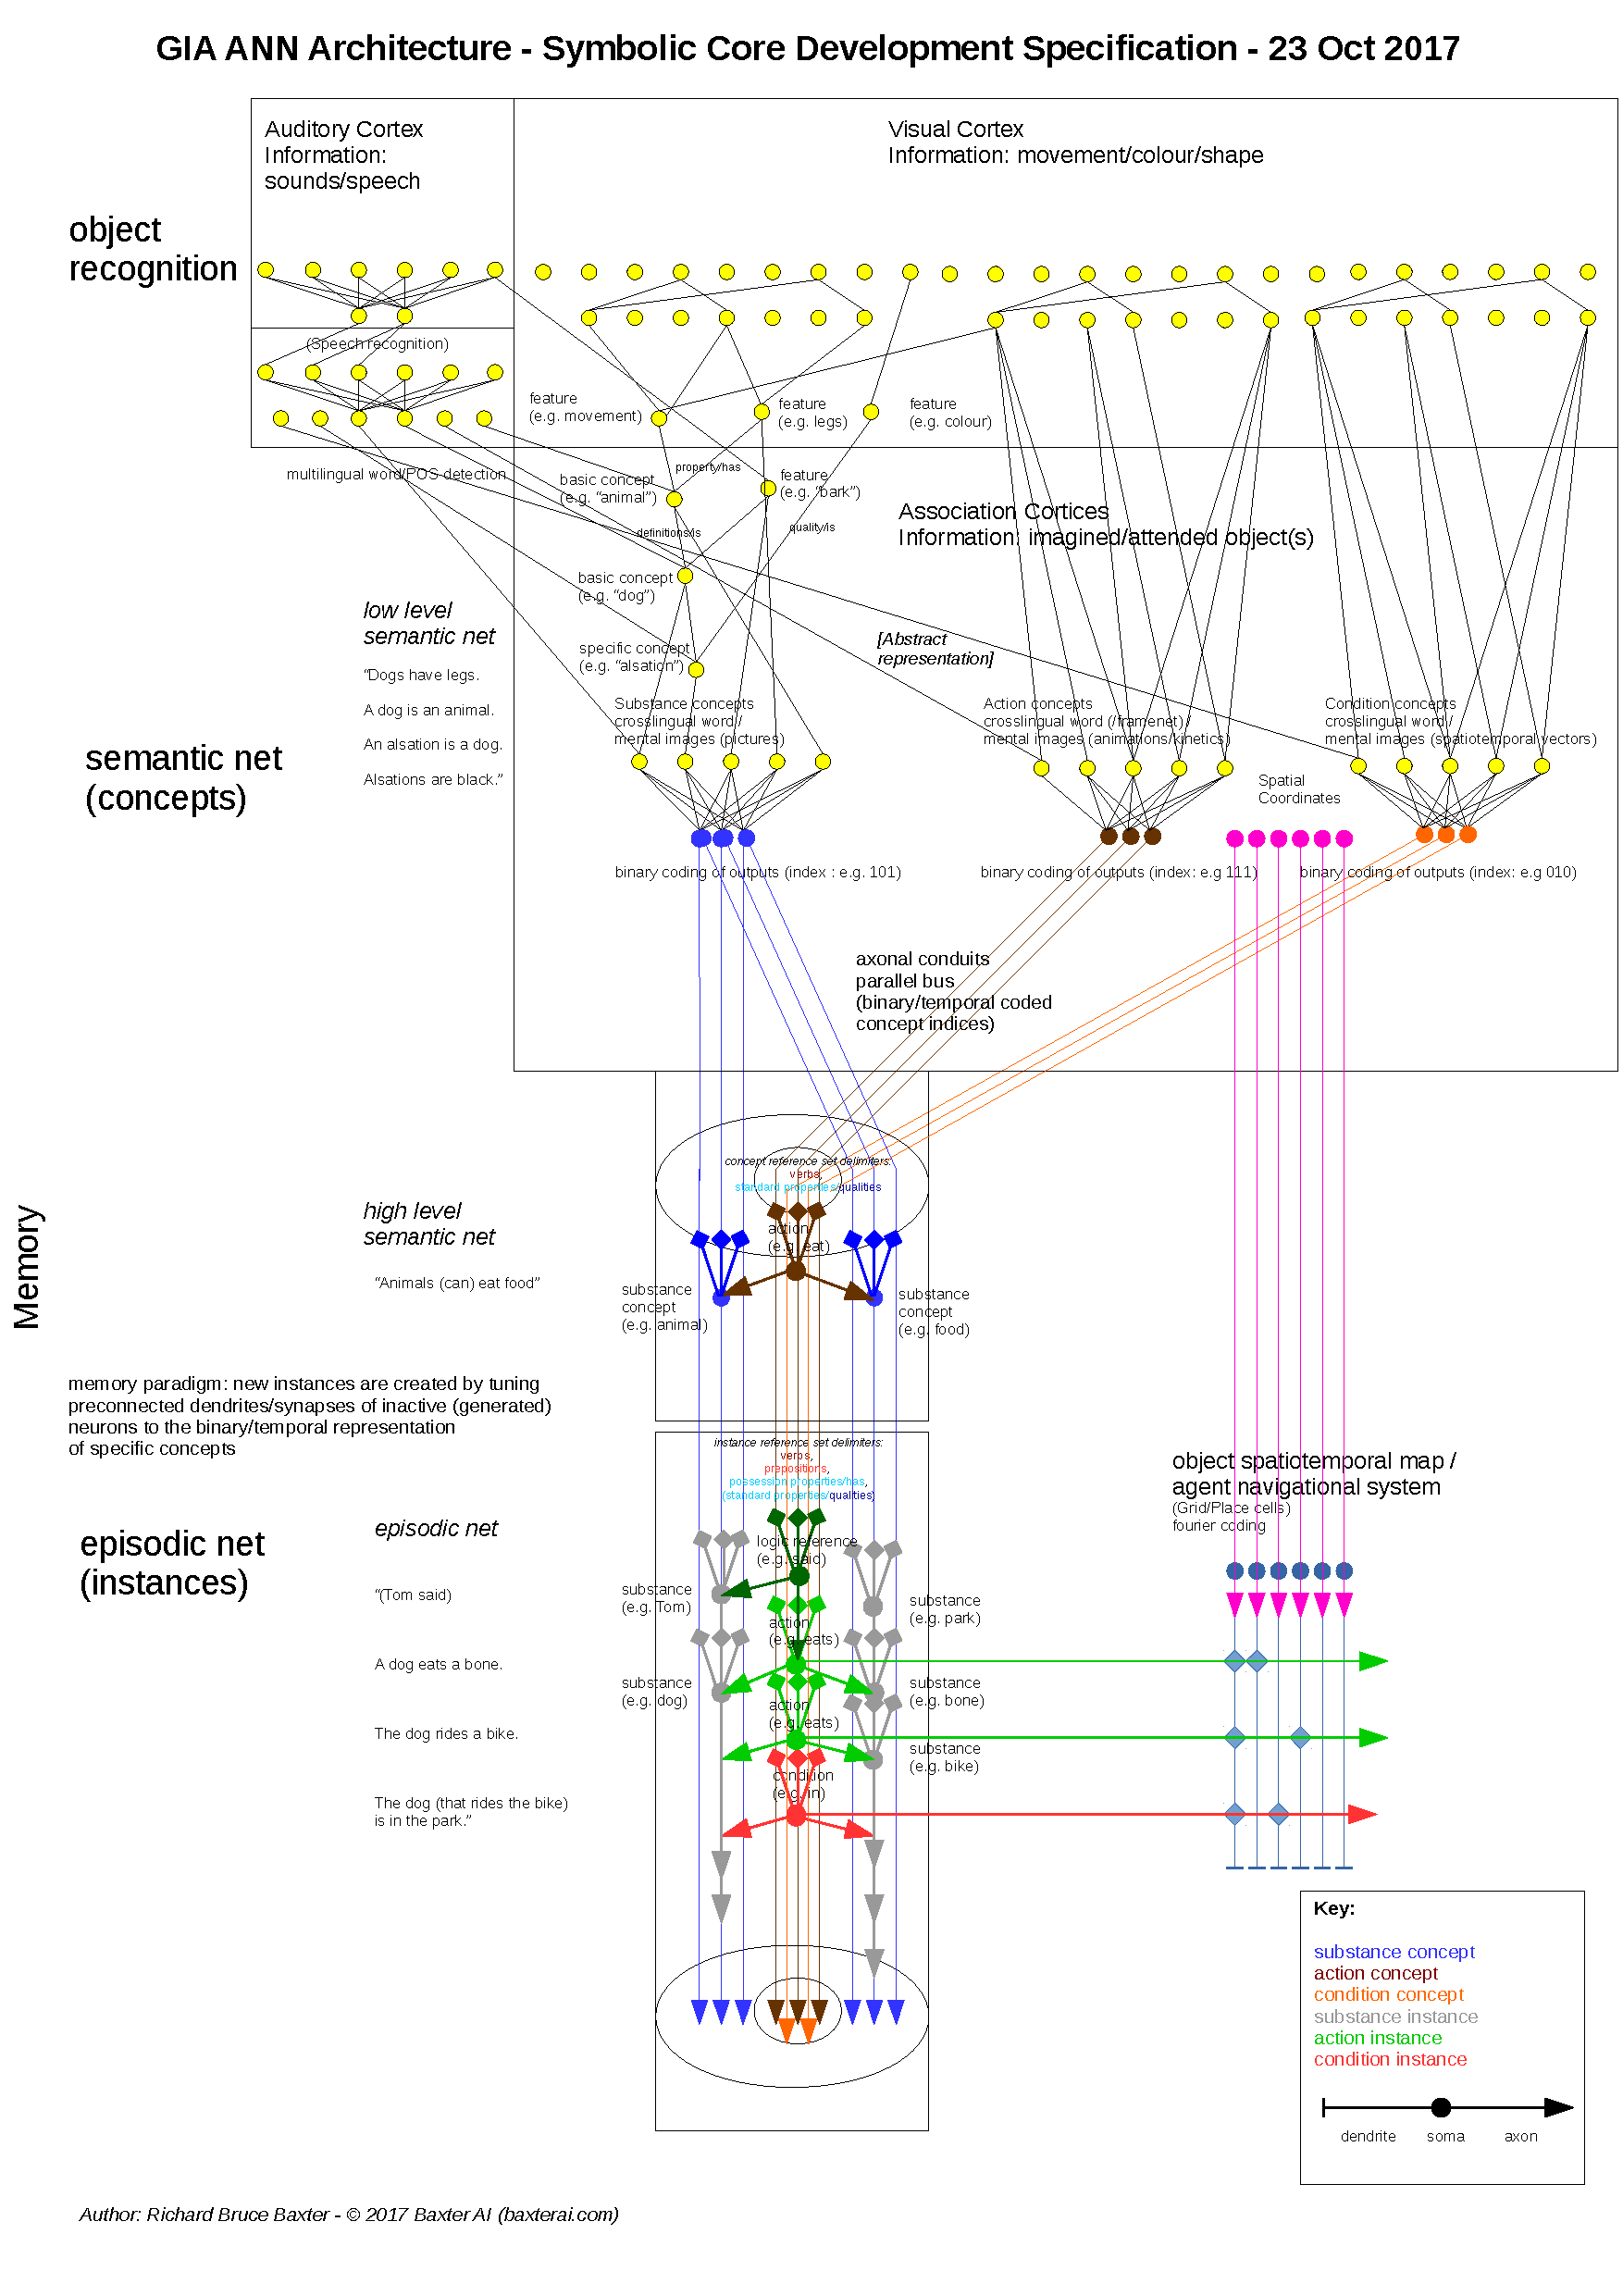
\includegraphics[width=\textwidth,height=0.88\textheight,keepaspectratio]{dev/GIAANNarchitectureDevelopment-23October2017a.pdf}
    \caption{Initial symbolic core with semantic concepts, episodic instances, and binary reference coding over axonal conduits.}
    \label{fig:dev-2017-initial-core}
\end{figure}
\clearpage

\begin{figure}[p]
    \centering
    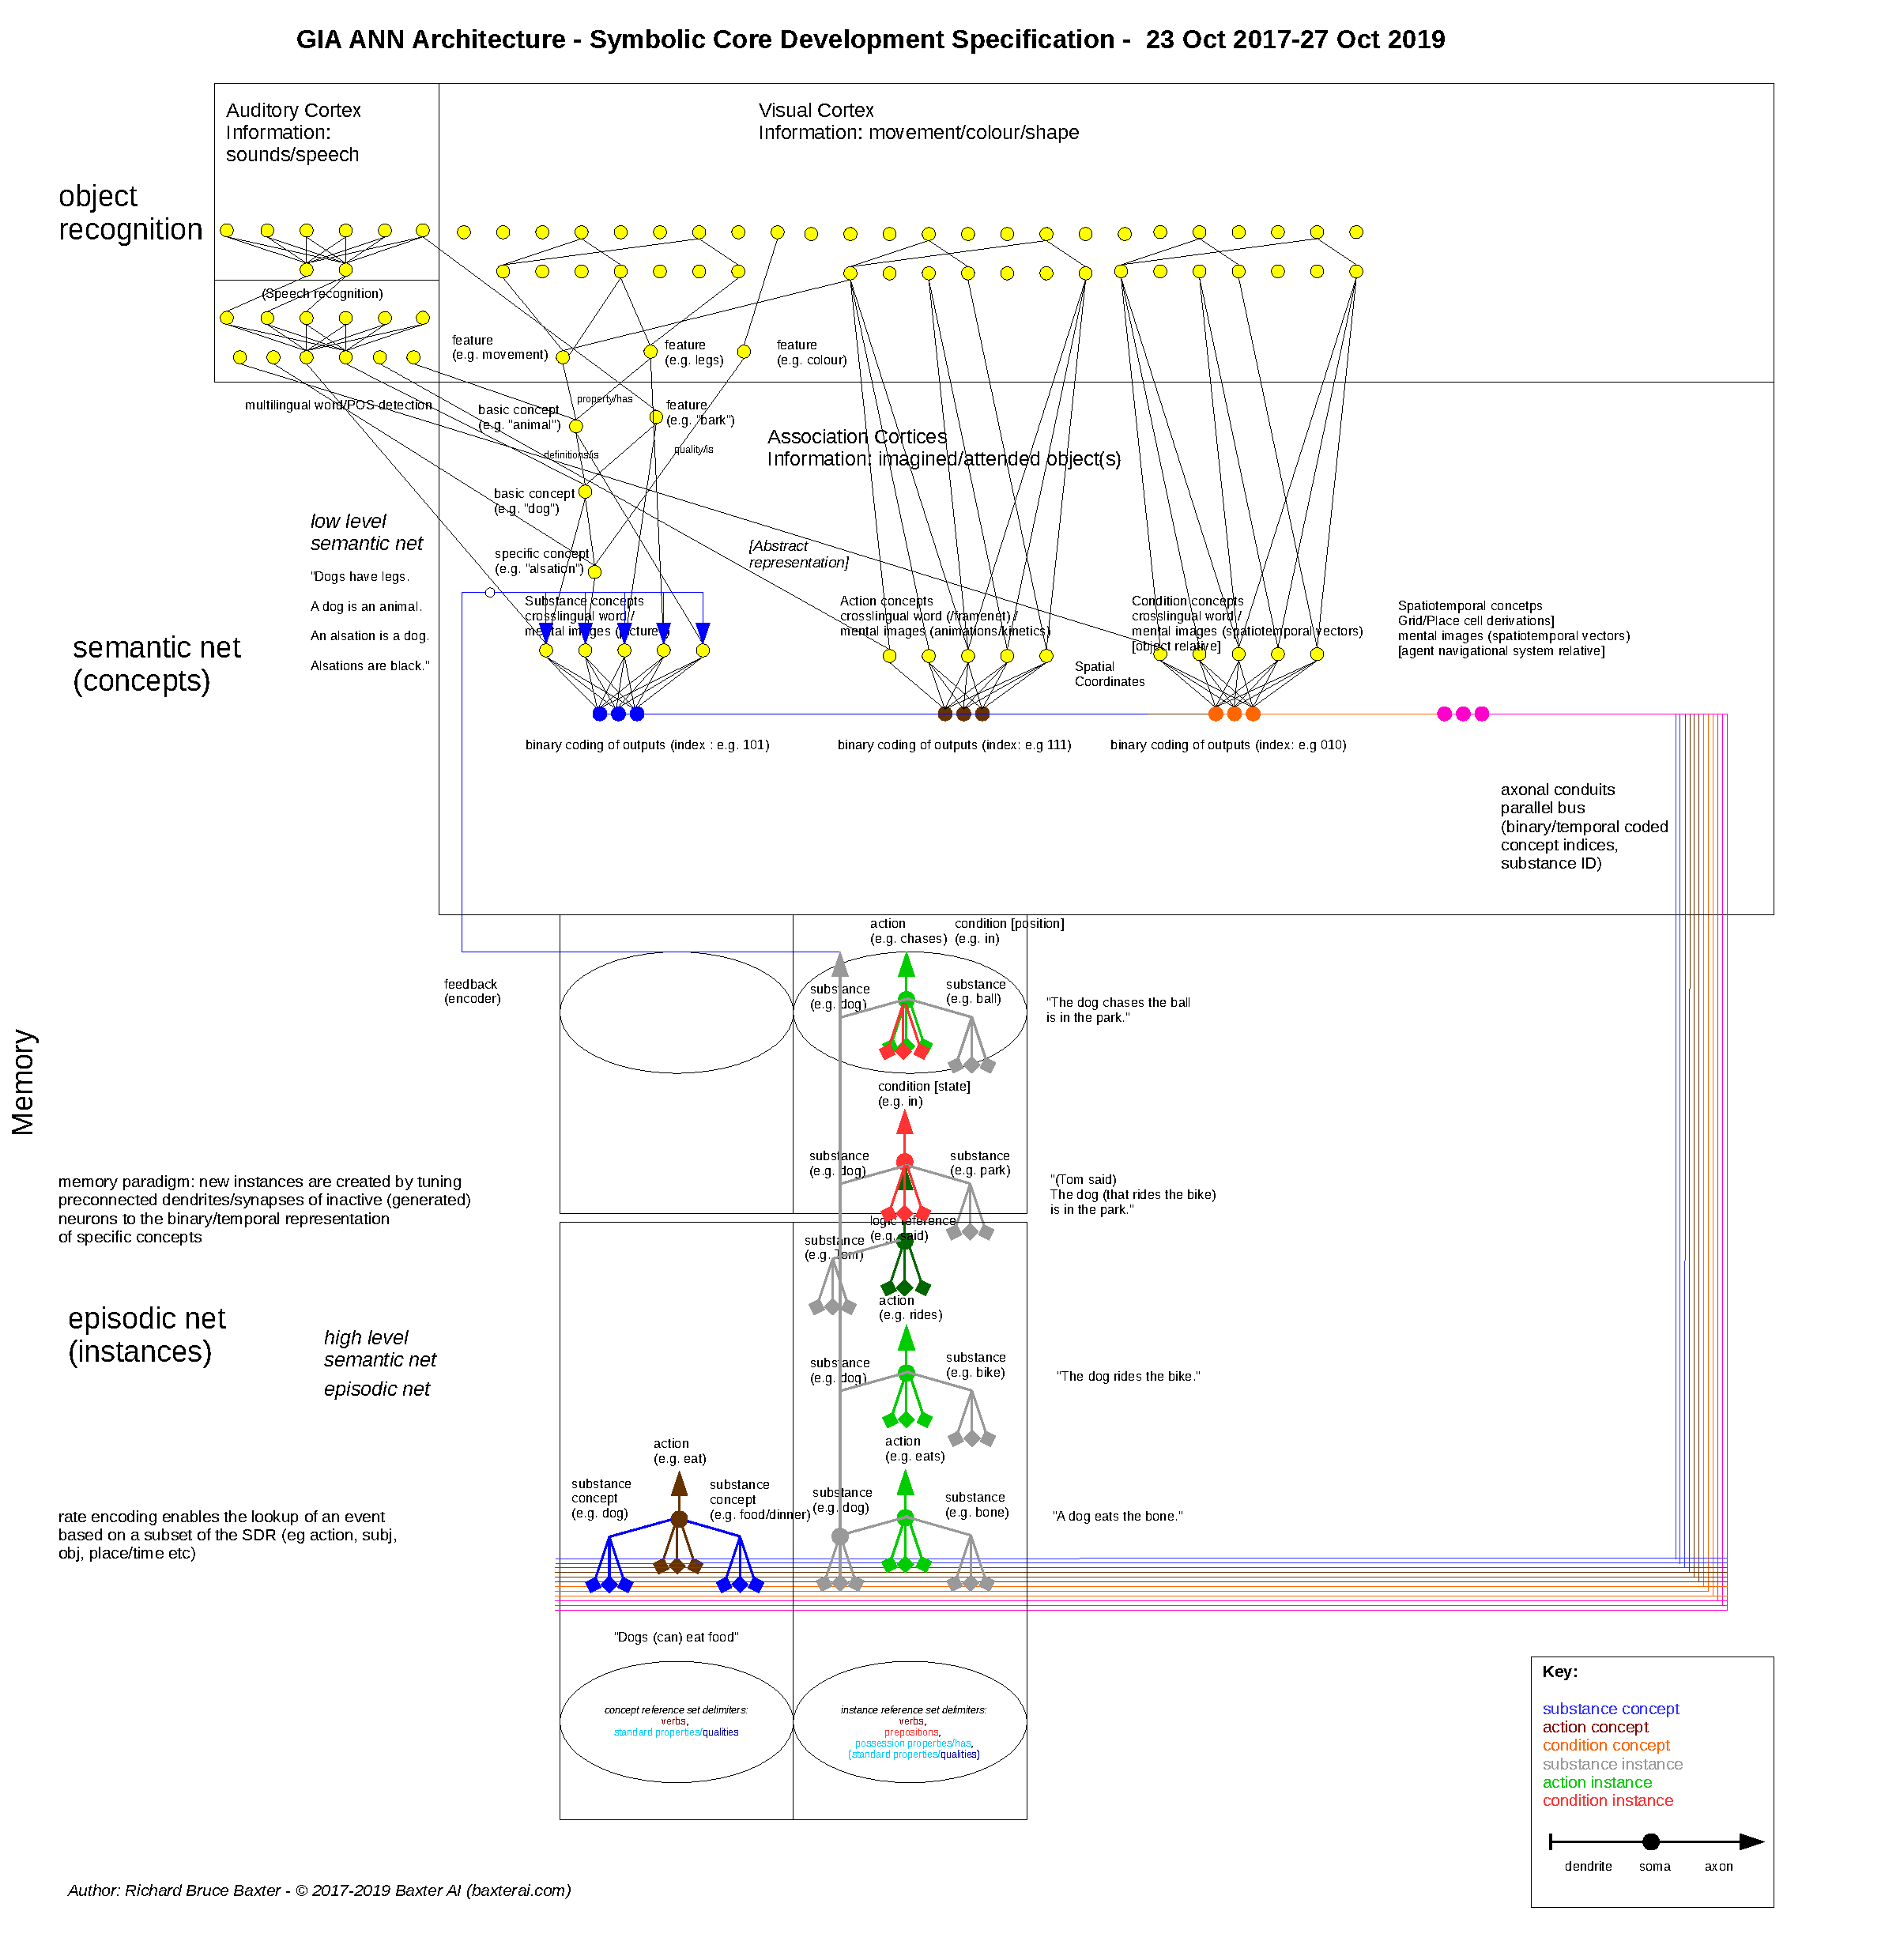
\includegraphics[width=\textwidth,height=0.88\textheight,keepaspectratio]{dev/GIAANNarchitectureDevelopment-27October2019a.pdf}
    \caption{Event retrieval refinement with feedback encoding and rate-coded lookup from partial cues (subject/action/object/place-time subsets).}
    \label{fig:dev-2019-event-retrieval}
\end{figure}
\clearpage

\begin{figure}[p]
    \centering
    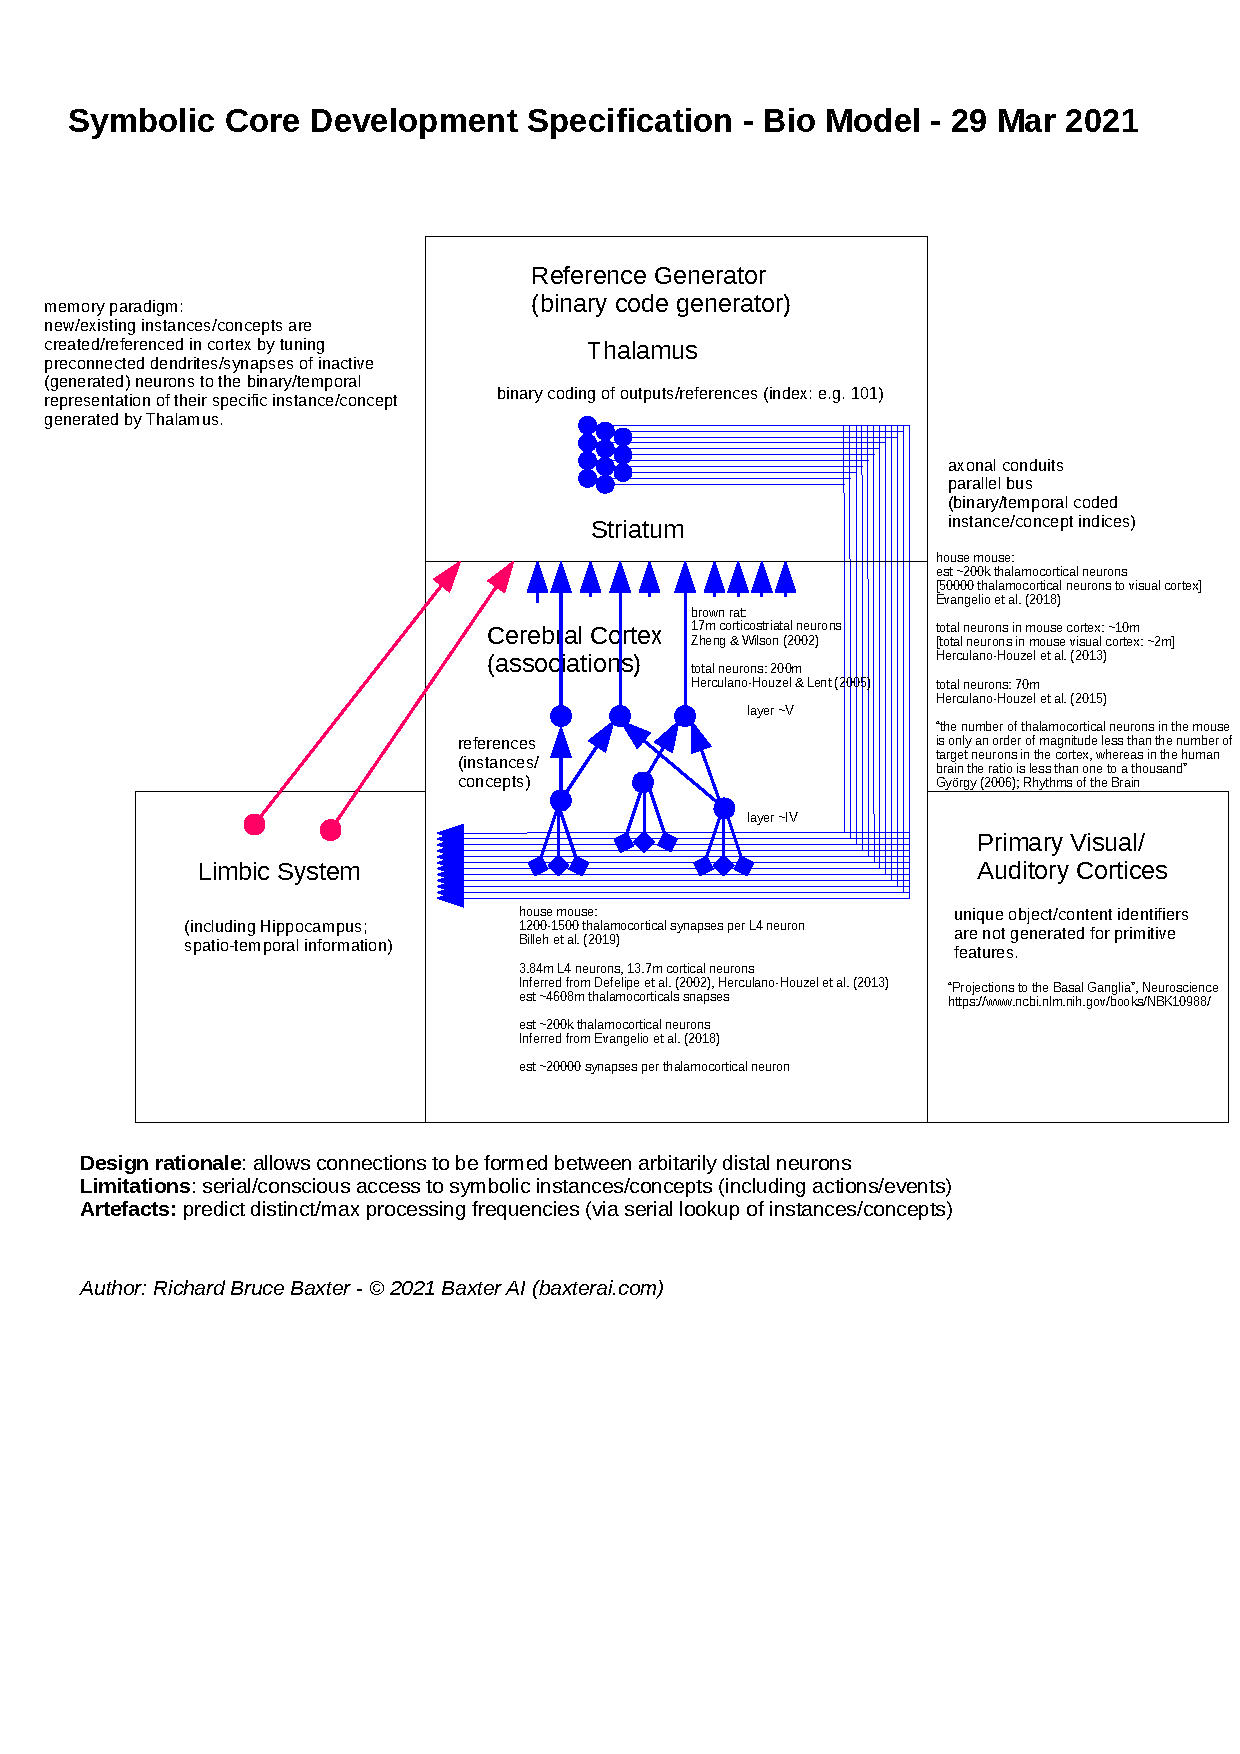
\includegraphics[width=\textwidth,height=0.88\textheight,keepaspectratio]{dev/GIAANNarchitectureDevelopment-bioModel-29March2021a.pdf}
    \caption{Bio-model mapping across thalamus, cortex, striatum, and limbic/hippocampal roles with design rationale and predicted serial-access constraints.}
    \label{fig:dev-2021-biomodel-mapping}
\end{figure}
\clearpage

\begin{figure}[p]
    \centering
    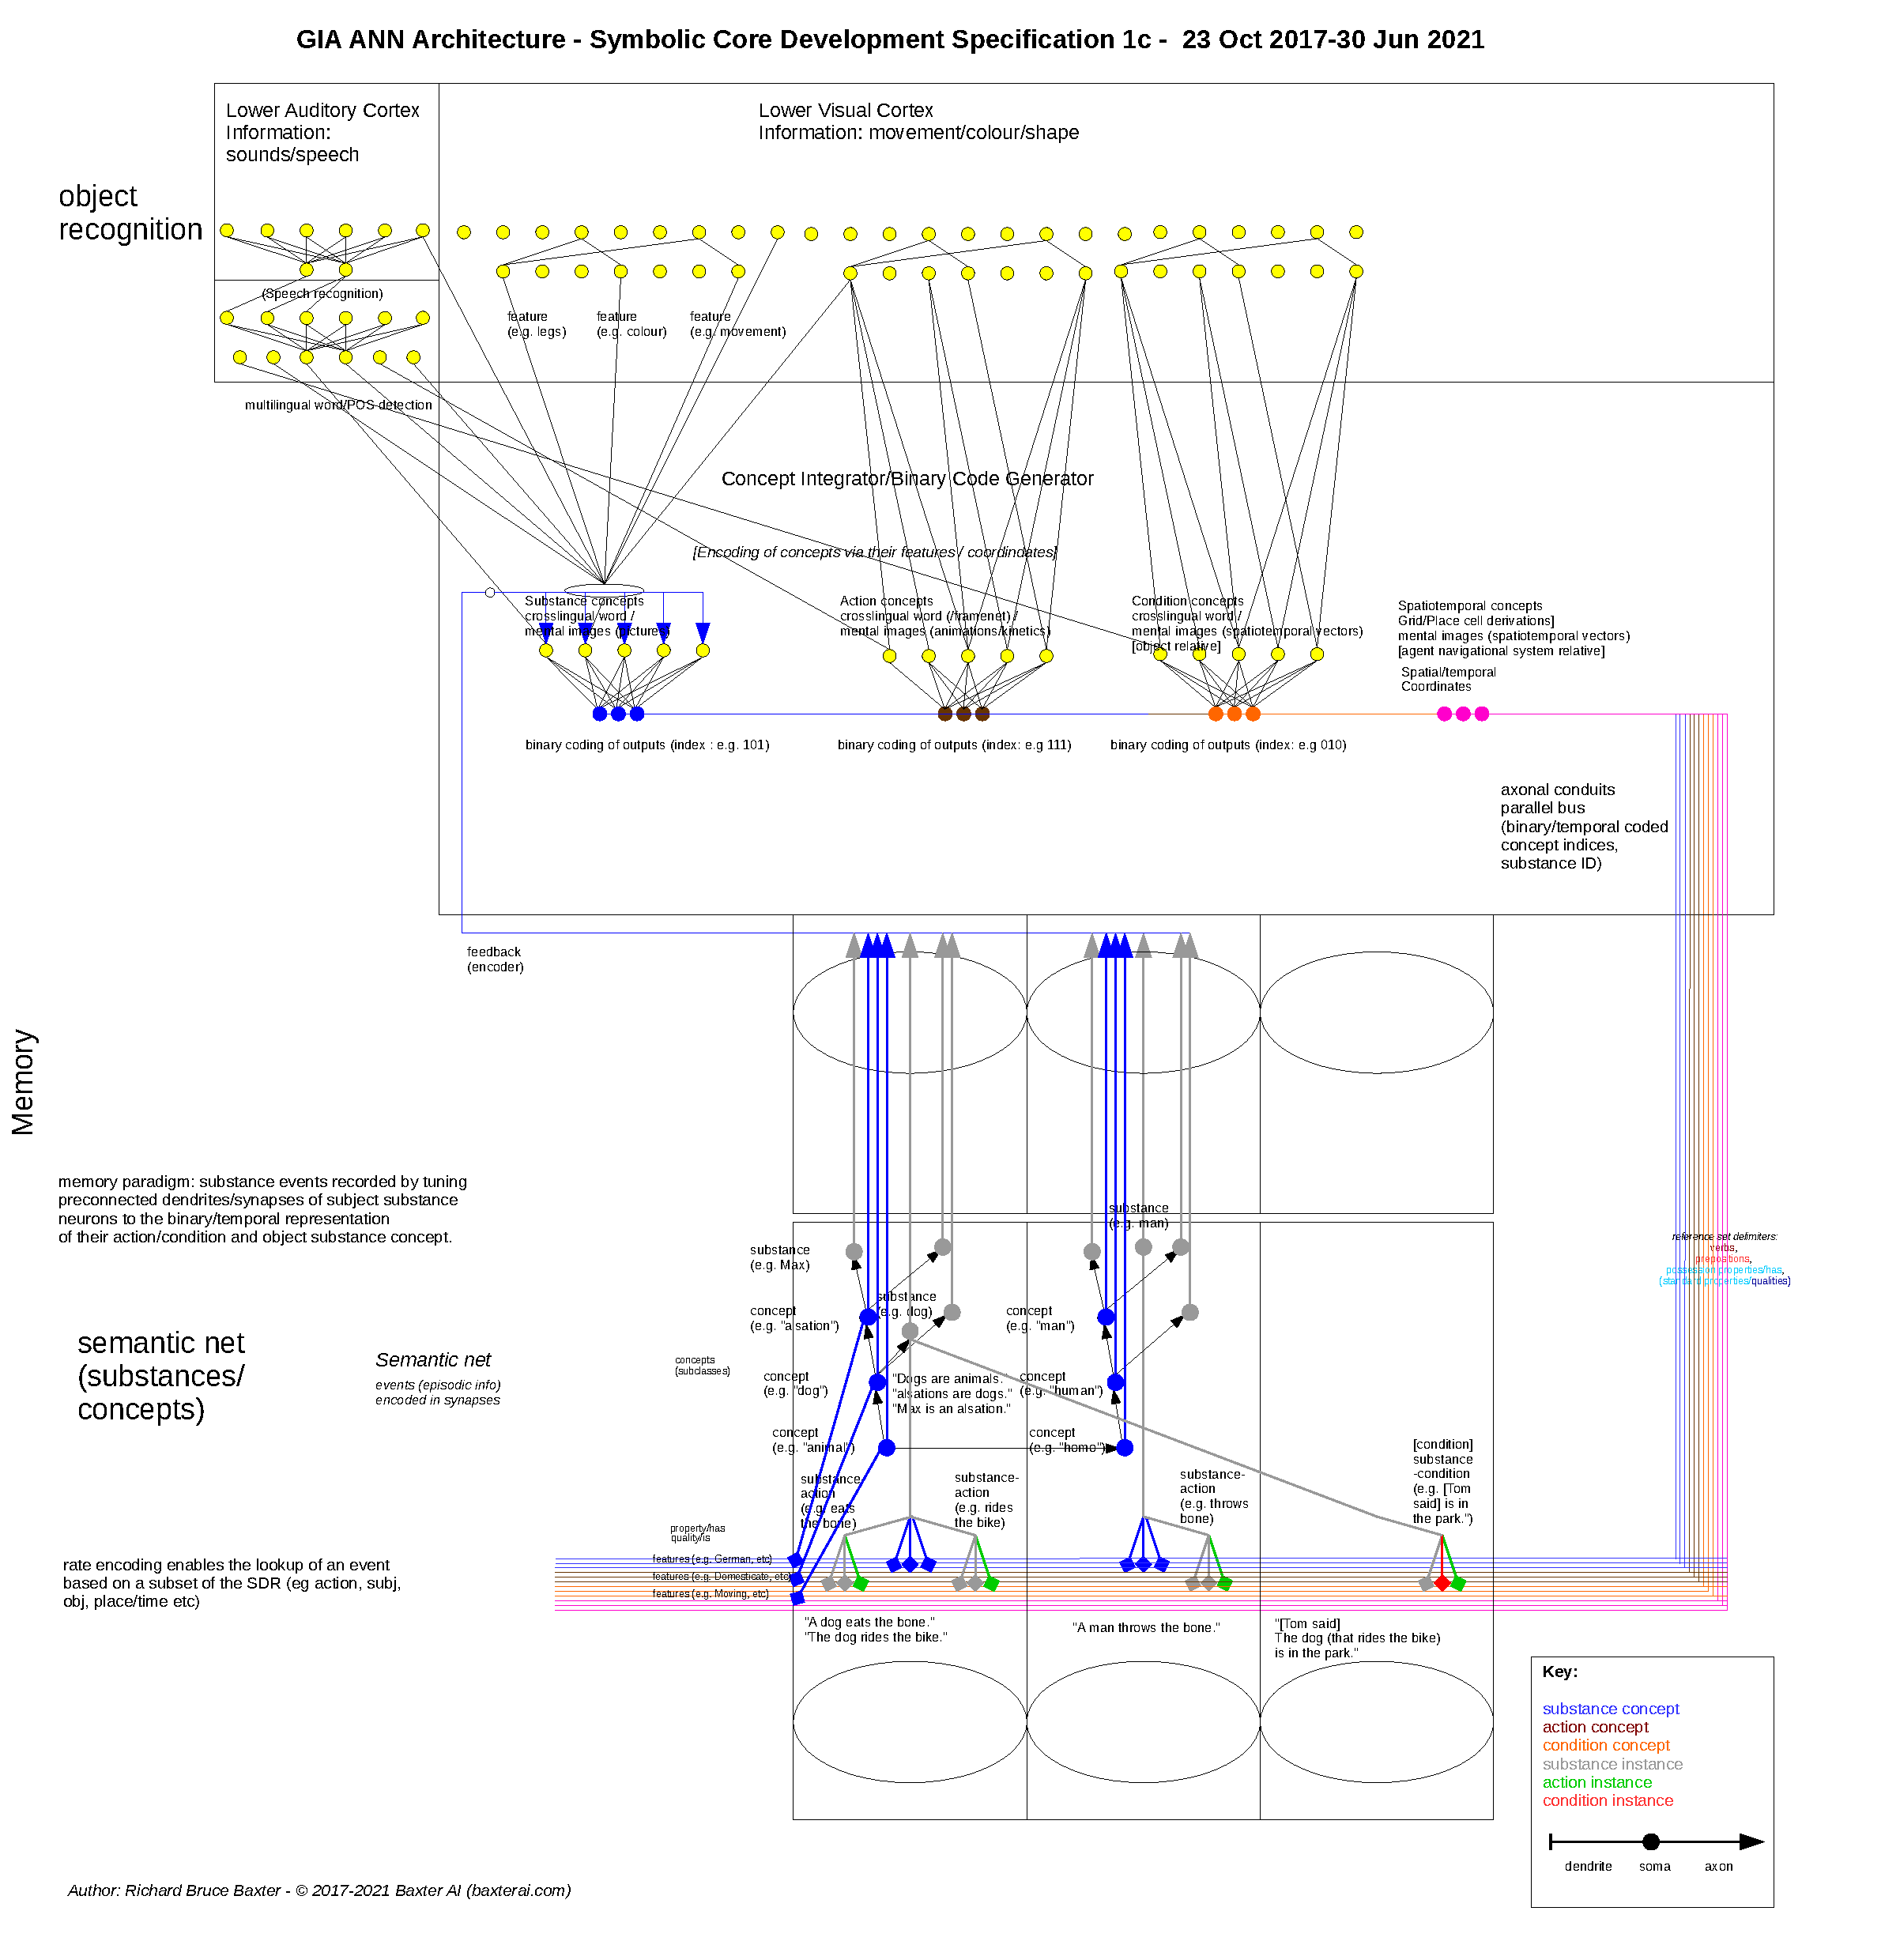
\includegraphics[width=\textwidth,height=0.88\textheight,keepaspectratio]{dev/GIAANNarchitectureDevelopment1c-30June2021a.pdf}
    \caption{Transition toward storing episodic information in synapses associated with substance/concept neurons, with a consolidated concept-integrator/reference-generator pathway.}
    \label{fig:dev-2021-synaptic-encoding}
\end{figure}
\clearpage

\begin{figure}[p]
    \centering
    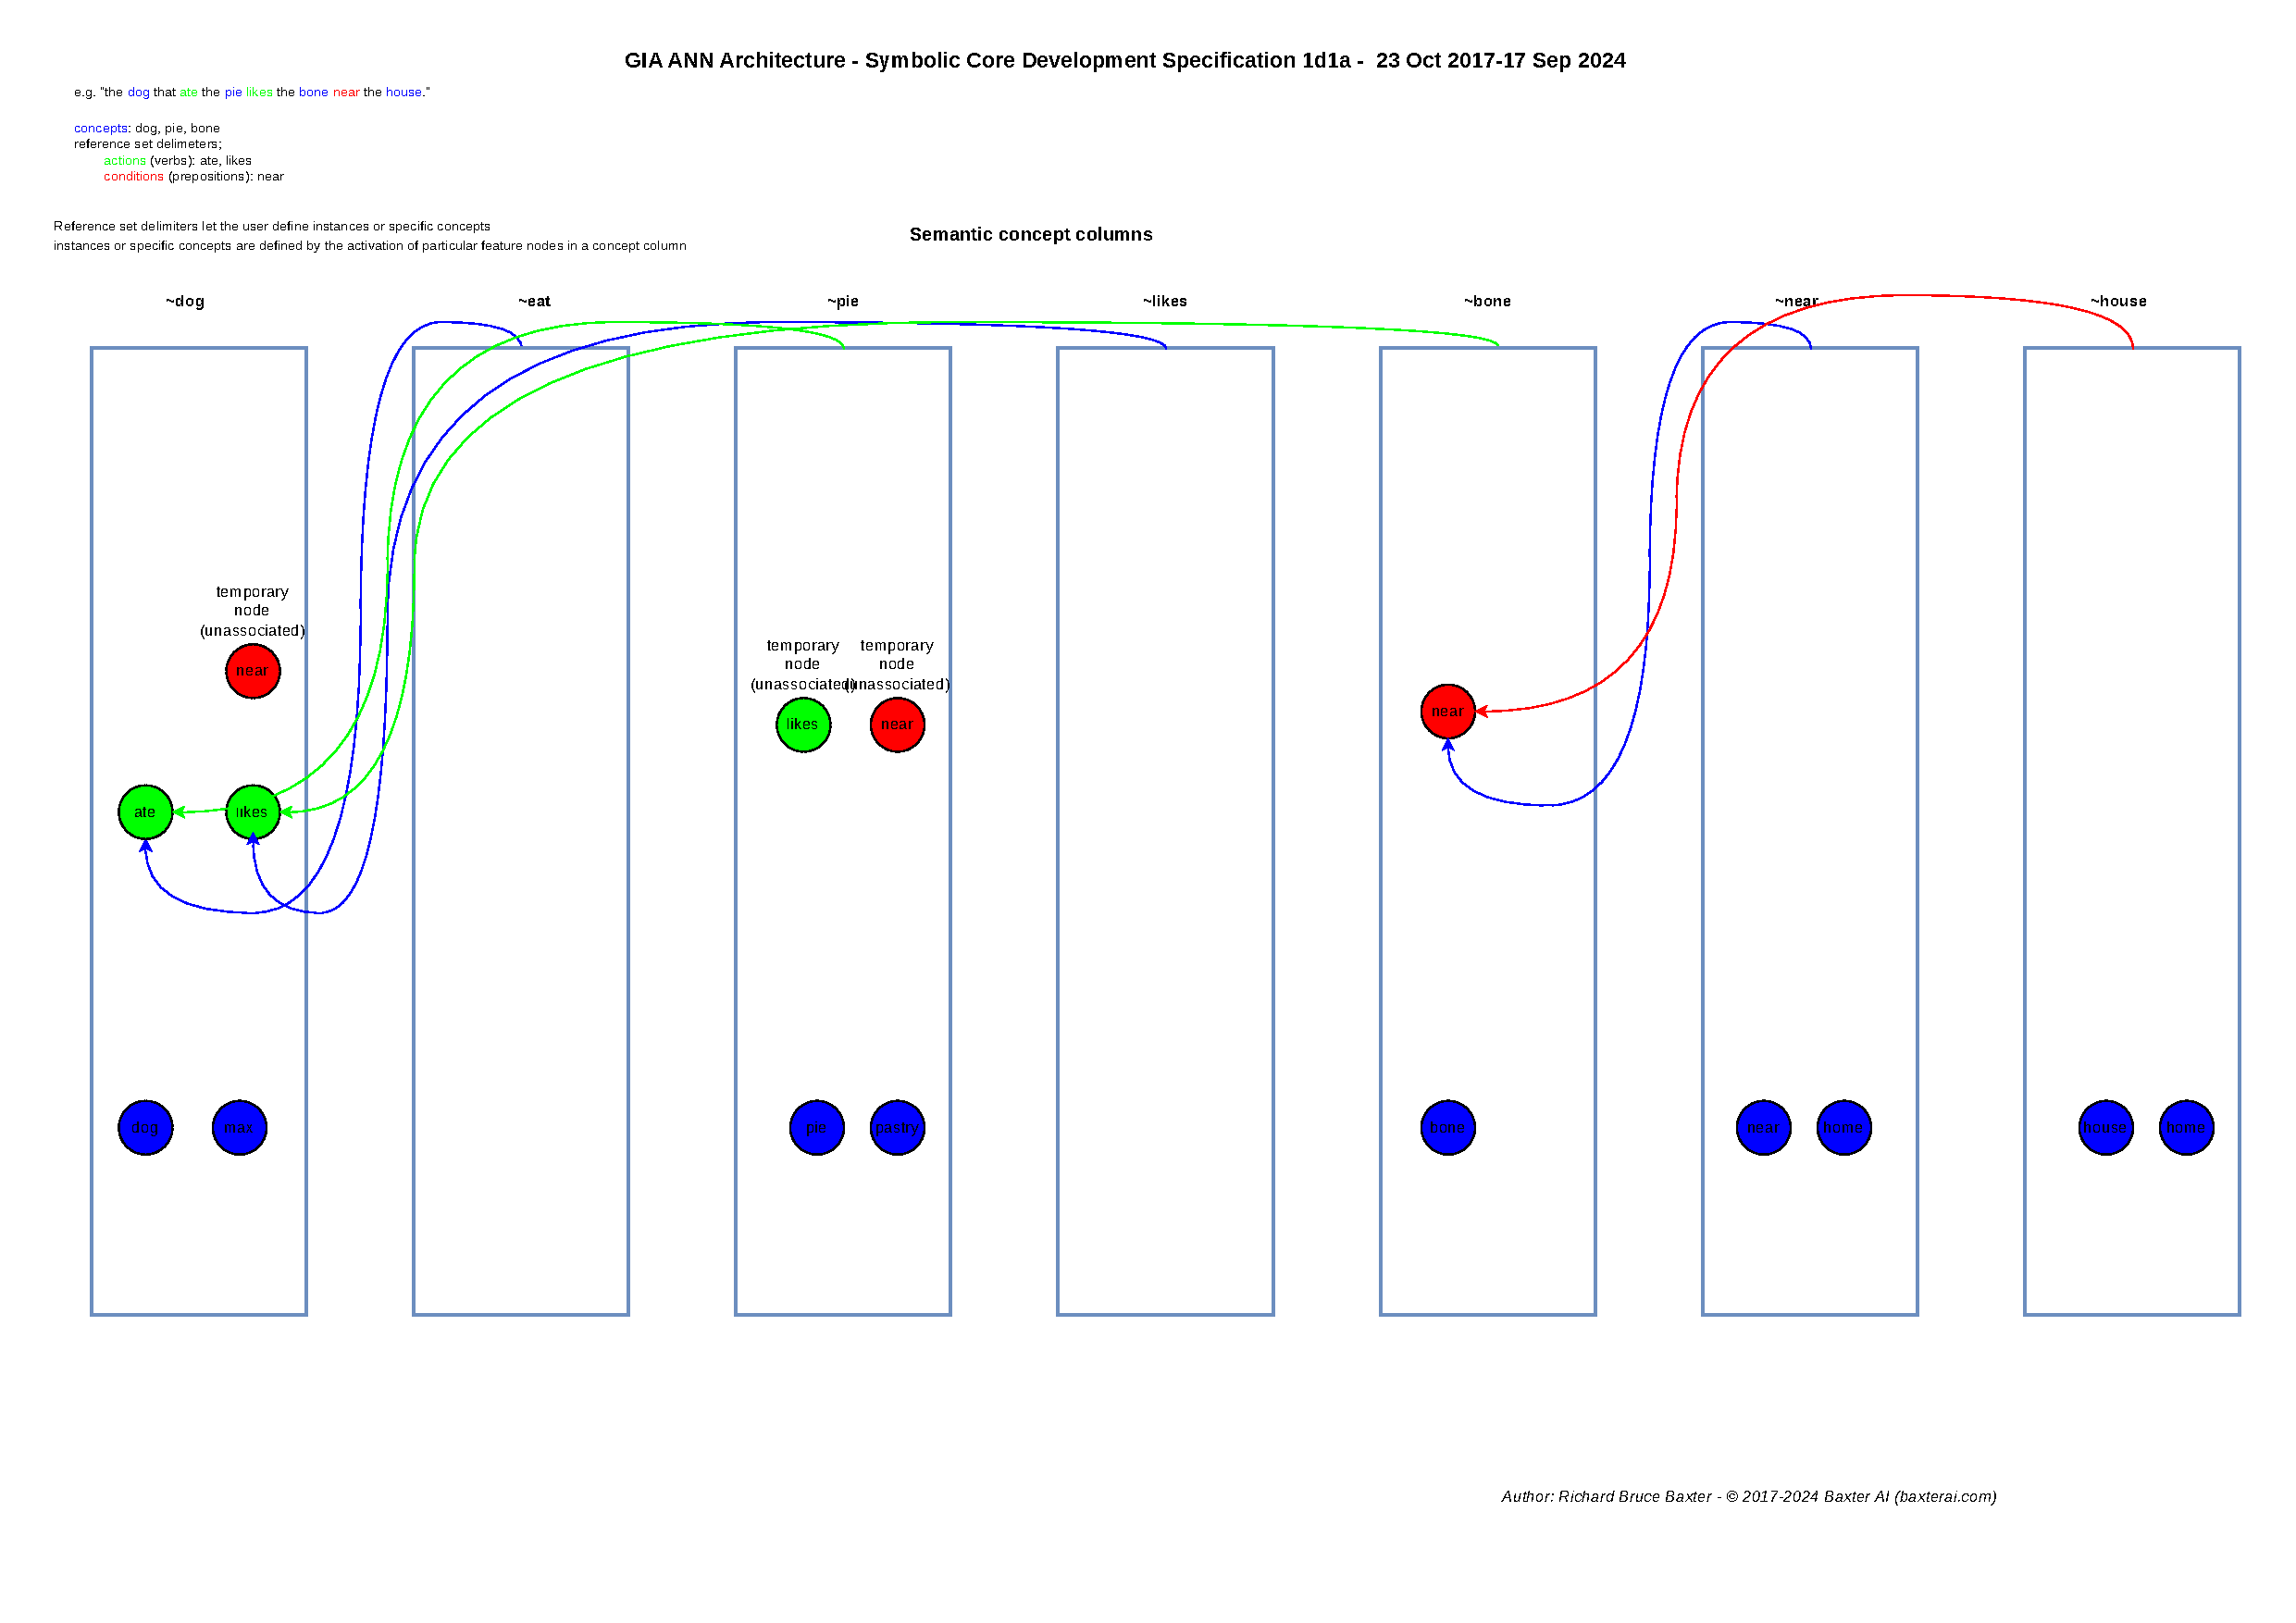
\includegraphics[width=\textwidth,height=0.88\textheight,keepaspectratio]{dev/GIAANNarchitectureDevelopment1d1a-17Sept2024a.pdf}
    \caption{Introduction of semantic concept columns and temporary unassociated nodes, with inter-column delimiter features (verbs and prepositions) used as routing constraints.}
    \label{fig:dev-2024-columns-routing}
\end{figure}
\clearpage

\begin{figure}[p]
    \centering
    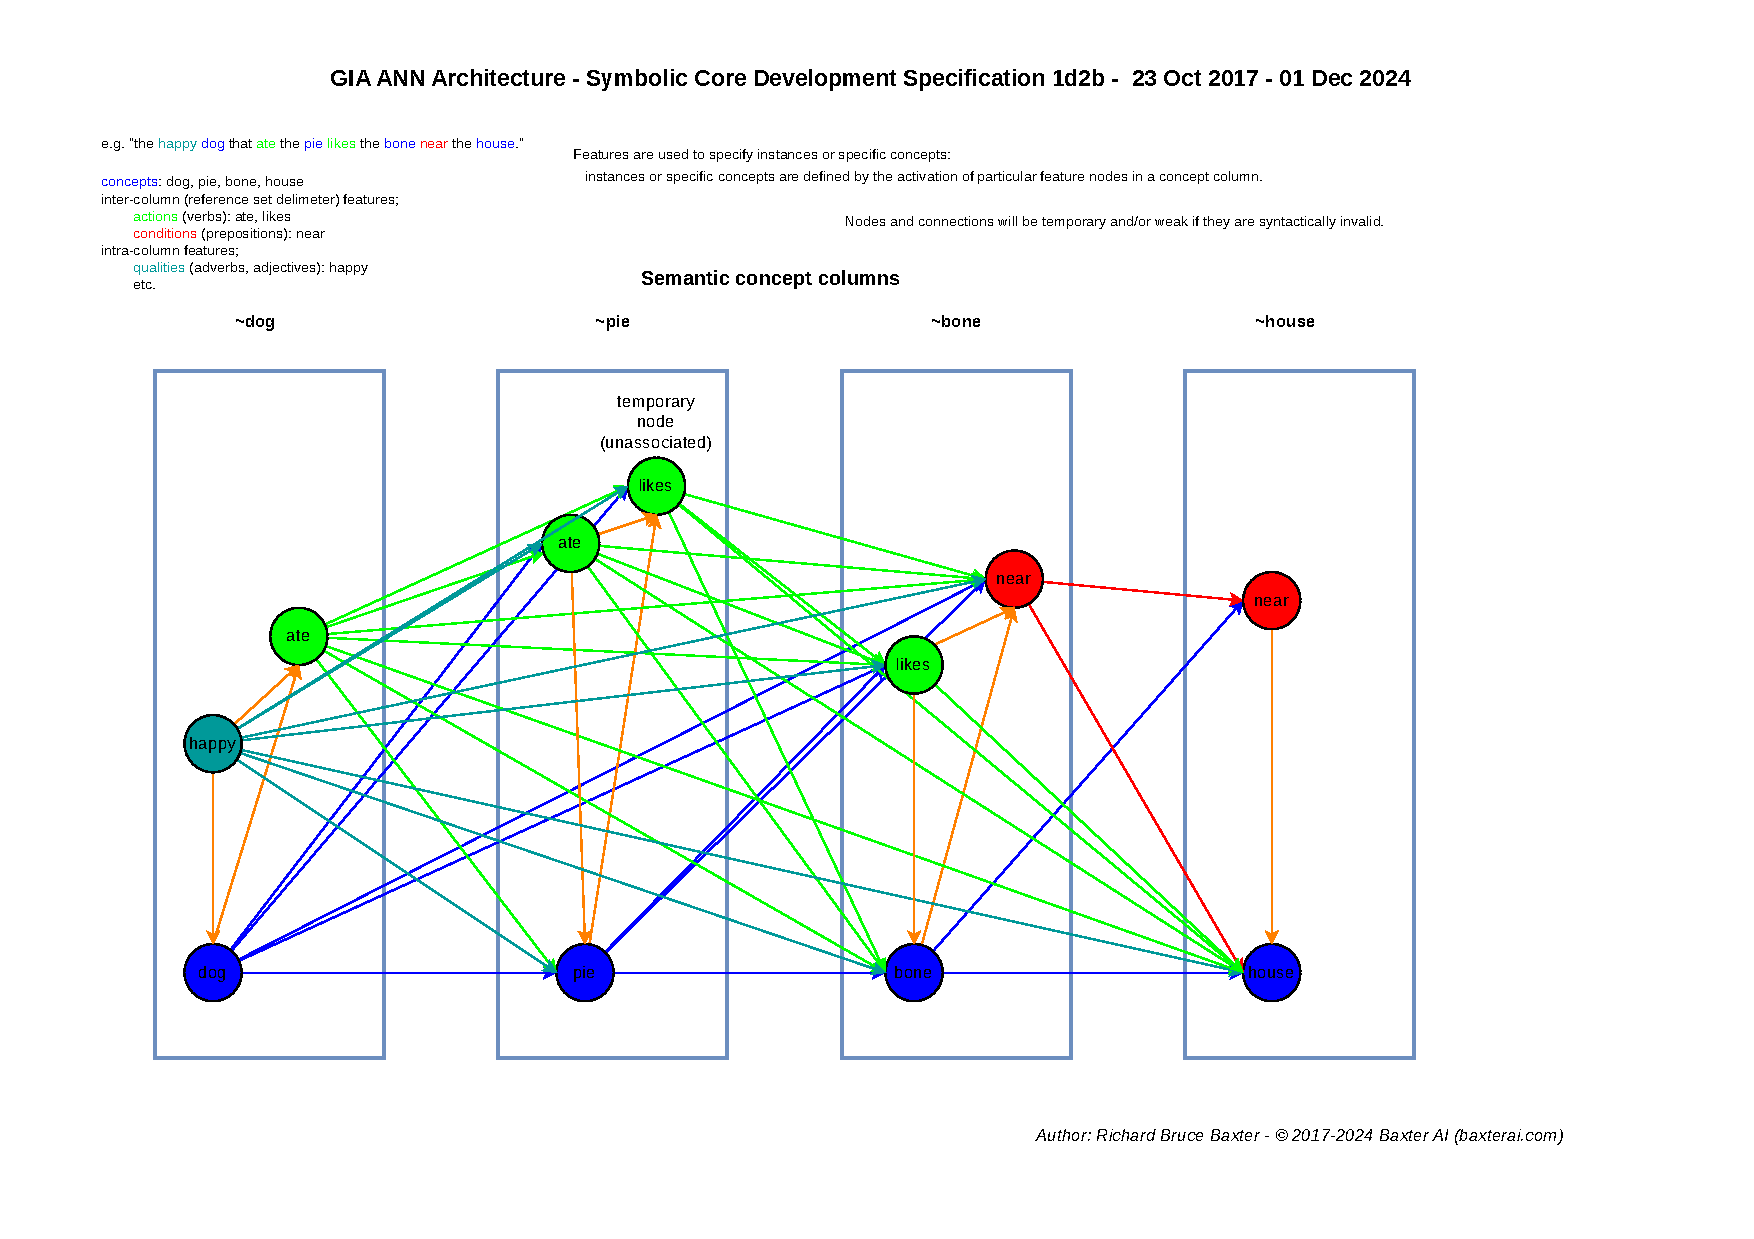
\includegraphics[width=\textwidth,height=0.88\textheight,keepaspectratio]{dev/GIAANNarchitectureDevelopment1d2b-01Dec2024a.pdf}
    \caption{Split between inter-column and intra-column features (e.g., qualities), plus syntactic-validity gating so invalid nodes/links remain weak or temporary.}
    \label{fig:dev-2024-feature-split-gating}
\end{figure}
\clearpage

\subsection{GIAANN Proto Specification}\label{subsec:appendix-giaann-proto-spec}

\noindent\textbf{File:} \texttt{dev/GIAANNproto1.nlc}

\lstinputlisting[
	language={},
	basicstyle=\scriptsize\rmfamily,
	breaklines=true,
	breakatwhitespace=true,
	columns=flexible,
	showstringspaces=false
]{dev/GIAANNproto1.nlc}

\end{document}